\chapter{RESULTS AND PERFORMANCE EVALUATION}

\section{Evaluation Metrics}

For a seven-class problem, let $TP_c$, $FP_c$ and $FN_c$ be the true positives,
false positives and false negatives of class $c$. Per-class precision, recall and
F1 are
\begin{equation}
  P_c = \frac{TP_c}{TP_c + FP_c}, \qquad
  R_c = \frac{TP_c}{TP_c + FN_c}, \qquad
  F1_c = \frac{2P_cR_c}{P_c + R_c},
  \label{eq:prf}
\end{equation}
and the two aggregations used in this report are
\begin{equation}
  \text{macro F1} = \frac{1}{K}\sum_{c=1}^{K} F1_c,
  \qquad
  \text{weighted F1} = \sum_{c=1}^{K}\frac{n_c}{N}\,F1_c ,
  \label{eq:aggregation}
\end{equation}
where $n_c$ is the number of test beans of class $c$. Accuracy is the trace of the
confusion matrix divided by $N$.

Macro F1 is the primary metric for two reasons. It weights every variety equally,
so a model cannot buy accuracy by sacrificing Bombay, which contributes only 3.84\%
of the beans; and it is a harmonic mean, so it punishes a model that achieves high
recall by predicting a class indiscriminately. Weighted F1 is reported alongside
it because it is the quantity a grading line actually experiences: it weights each
bean equally, so errors on the large classes count more. When the two diverge, the
difference localises the errors, and that is exactly what happens in
Table~\ref{tab:model_comparison}, where macro F1 exceeds accuracy for every model.

ROC-AUC is computed with the one-vs-rest strategy: for each variety, the
probability of that variety is treated as a score against all other varieties
combined, and the area under the resulting curve is averaged over the seven
classes. It measures ranking quality independently of the decision threshold,
which matters if the model is later given a rejection option.

\section{Experimental Results}

Table~\ref{tab:model_comparison} reports the held-out performance of all six
models, and Table~\ref{tab:cv_results} reports the cross-validated scores that
were used to select them. Figure~\ref{fig:comparison} shows the three main metrics
side by side.

\begin{table}[htbp]
\centering
\scriptsize
\caption{Performance on the 2,723-bean held-out test set. Rows are ordered by test macro F1}
\label{tab:model_comparison}
\begin{tabular}{lrrrrrr}
\toprule
Model & Accuracy & Macro prec. & Macro rec. & Macro F1 & Weighted F1 & ROC-AUC \\
\midrule
RBF-SVM & 0.9258 & 0.9383 & 0.9362 & 0.9372 & 0.9258 & 0.9953 \\
Hist Gradient Boosting & 0.9229 & 0.9368 & 0.9328 & 0.9347 & 0.9229 & 0.9948 \\
Logistic Regression & 0.9214 & 0.9357 & 0.9323 & 0.9337 & 0.9217 & 0.9949 \\
Extra Trees & 0.9207 & 0.9356 & 0.9306 & 0.9328 & 0.9208 & 0.9943 \\
Random Forest & 0.9196 & 0.9334 & 0.9297 & 0.9314 & 0.9195 & 0.9936 \\
K-Nearest Neighbours & 0.9174 & 0.9328 & 0.9279 & 0.9300 & 0.9175 & 0.9870 \\
\bottomrule
\end{tabular}
\end{table}


\begin{table}[htbp]
\centering
\footnotesize
\caption{Cross-validated macro F1 on the training partition (5 stratified folds). Sorted by mean macro F1}
\label{tab:cv_results}
\begin{tabular}{llcrrrrr}
\toprule
Model & Search & Configs & Mean & Std. dev. & Min & Max & Time (s) \\
\midrule
RBF-SVM & grid & 16 & 0.9444 & 0.0056 & 0.9391 & 0.9516 & 7.4 \\
Hist Gradient Boosting & random & 20 & 0.9424 & 0.0049 & 0.9379 & 0.9506 & 71.6 \\
K-Nearest Neighbours & grid & 40 & 0.9382 & 0.0048 & 0.9324 & 0.9426 & 4.1 \\
Random Forest & random & 25 & 0.9375 & 0.0037 & 0.9352 & 0.9440 & 183.9 \\
Logistic Regression & grid & 5 & 0.9374 & 0.0048 & 0.9321 & 0.9425 & 2.7 \\
Extra Trees & random & 25 & 0.9344 & 0.0033 & 0.9316 & 0.9402 & 24.4 \\
\bottomrule
\end{tabular}
\end{table}


\begin{figure}[htbp]
\centering
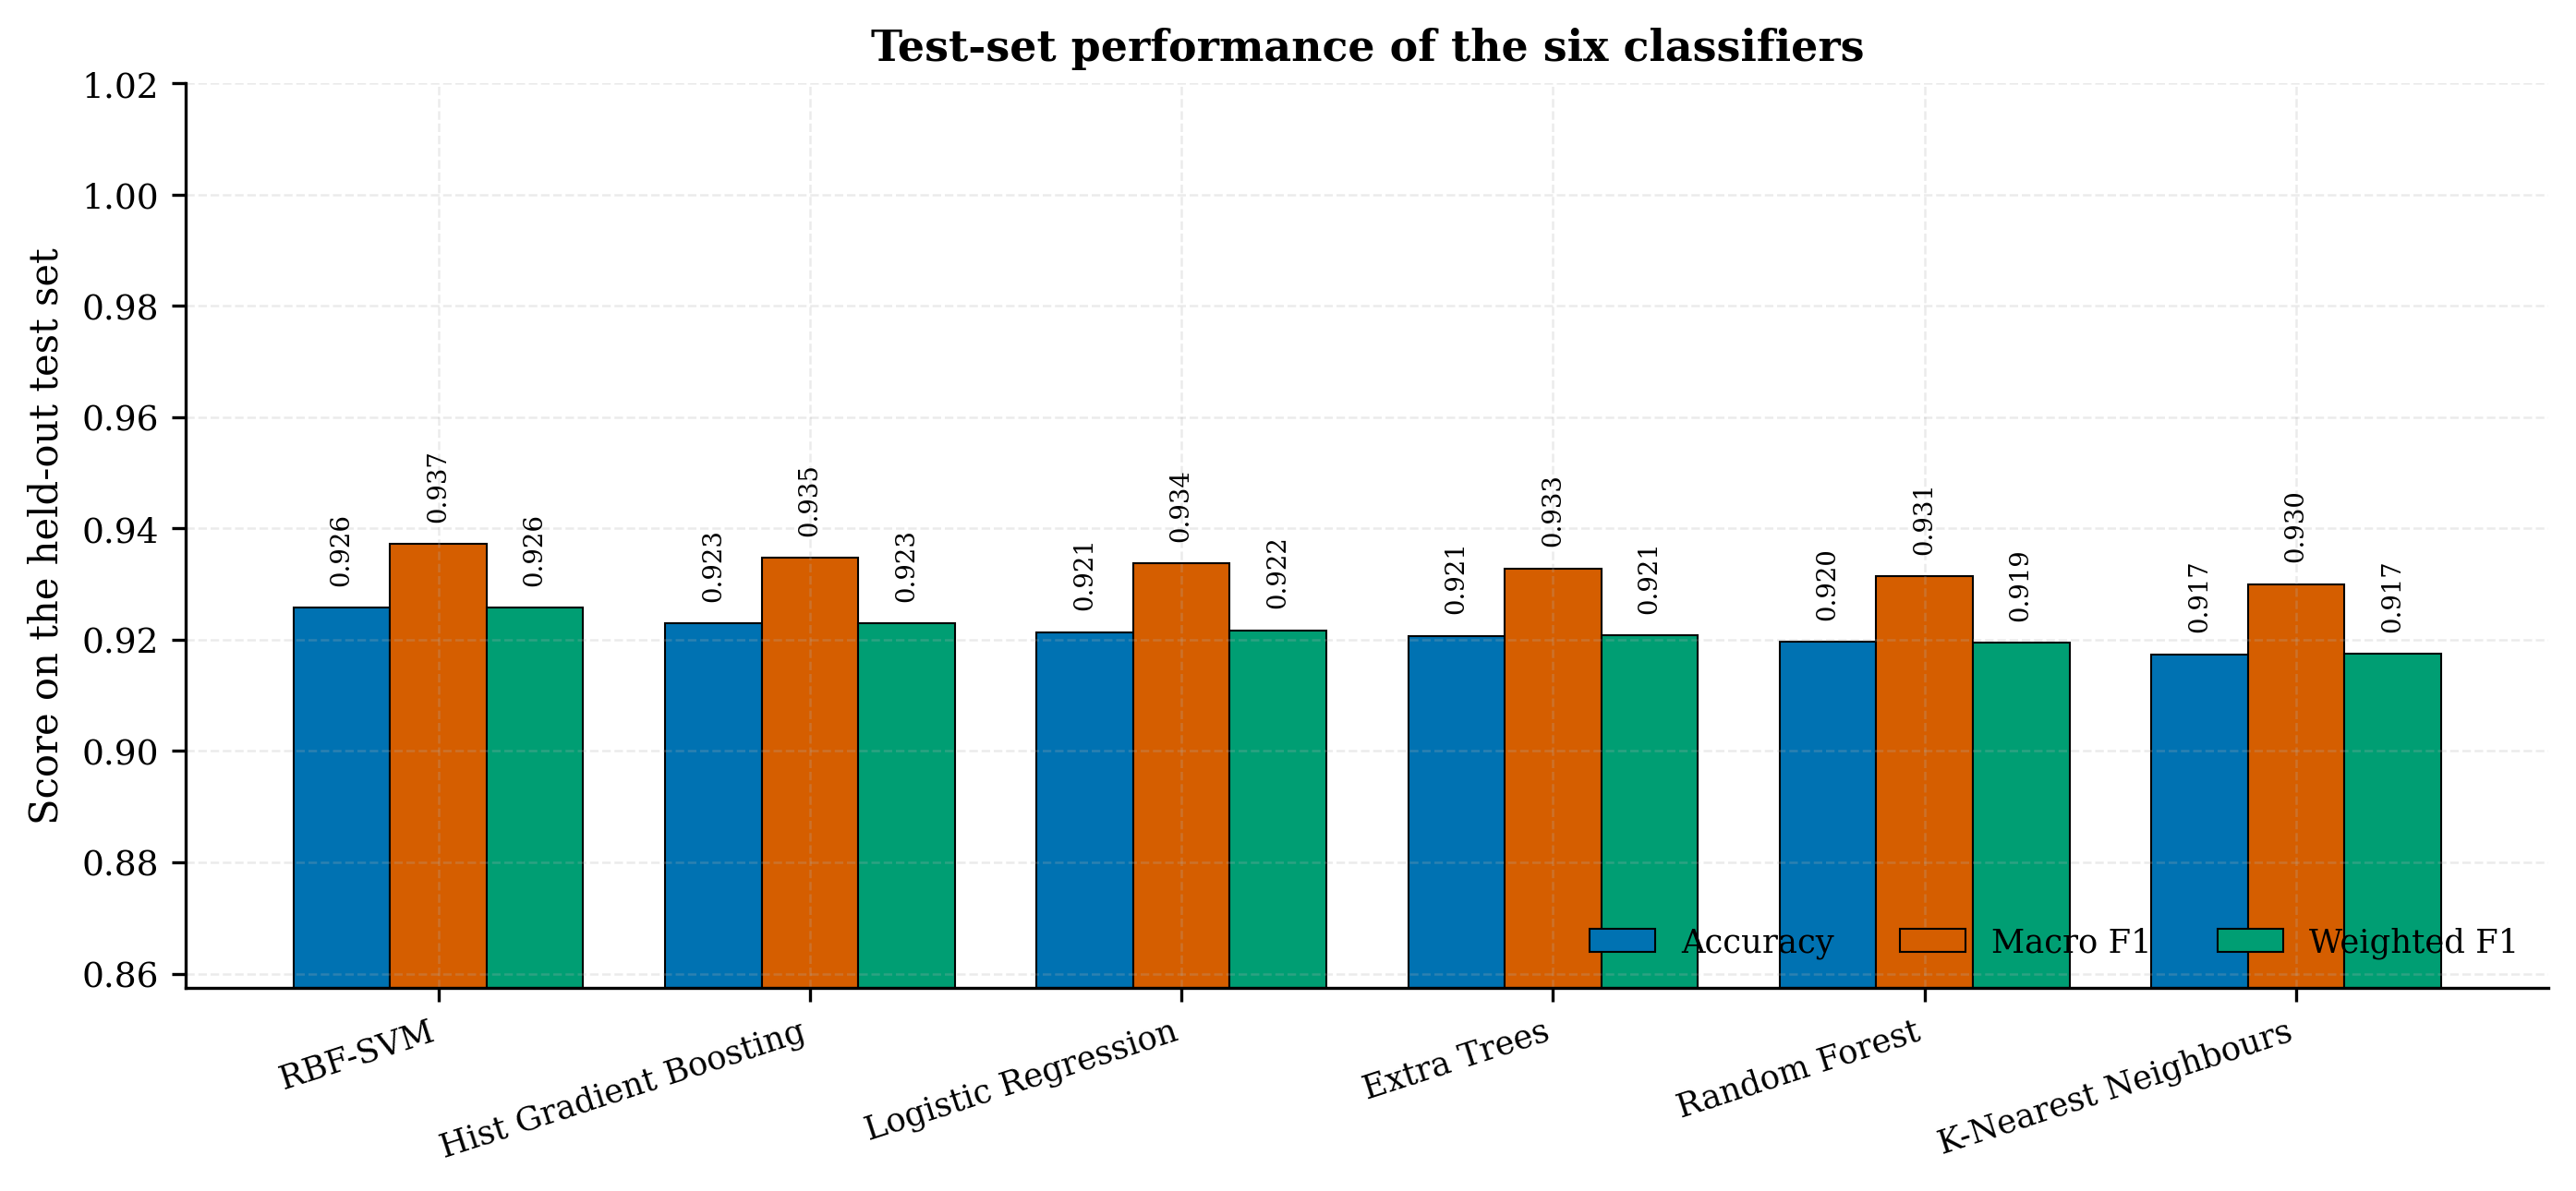
\includegraphics[width=0.82\textwidth]{fig_6_1_model_comparison.png}
\caption{Held-out accuracy, macro F1 and weighted F1 for the six classifiers. The
ordering is stable across the three metrics.}
\label{fig:comparison}
\end{figure}

The \BestModel{} leads on every metric: \BestAcc{} accuracy, \BestFOne{} macro F1,
\BestPrec{} macro precision, \BestRec{} macro recall and \BestAUC{} one-vs-rest
ROC-AUC. Histogram gradient boosting is second at \SecondFOne{} macro F1, and
k-nearest neighbours is last at \WorstFOne{}. The full spread from first to last
is 0.0072 macro F1, which corresponds to about 20 beans out of 2,723.

Two features of this table deserve comment before any interpretation.

First, macro F1 exceeds accuracy for all six models. This is not a paradox. The
two largest classes, Sira (527 test beans) and Dermason (709), carry most of the
errors, so they depress accuracy, which counts beans; Bombay, which is perfectly
classified, and Horoz and Seker, which are nearly so, raise the macro average,
which counts classes. A model with 0.9372 macro F1 and 0.9258 accuracy is
therefore a model that is excellent on five varieties and merely good on the two
largest ones.

Second, the cross-validated ranking in Table~\ref{tab:cv_results} is not the same
as the test ranking. k-nearest neighbours is third on cross-validation (0.9382) but
last on the test set (0.9300), while Extra Trees is last on cross-validation
(0.9344) but fourth on the test set (0.9328). The differences among the five
non-SVM models are between 0.002 and 0.004 macro F1, which is smaller than the
fold-to-fold standard deviation of 0.003 to 0.006 reported in the same table. The
honest reading is that those five models are statistically indistinguishable on
this dataset, and that their relative order on a single 2,723-bean test set is
partly noise. Only the SVM's advantage over the bottom of the table is larger than
the fold variance, and even that is modest.

\section{Visual Results}

Figure~\ref{fig:cmgrid} shows the six confusion matrices. The dominant feature is
common to all of them: the block formed by Sira and Dermason. In every model the
largest off-diagonal entries are Sira predicted as Dermason and Dermason predicted
as Sira. Bombay is classified perfectly by all six models, and Horoz and Seker are
almost always correct.

\begin{figure}[htbp]
\centering
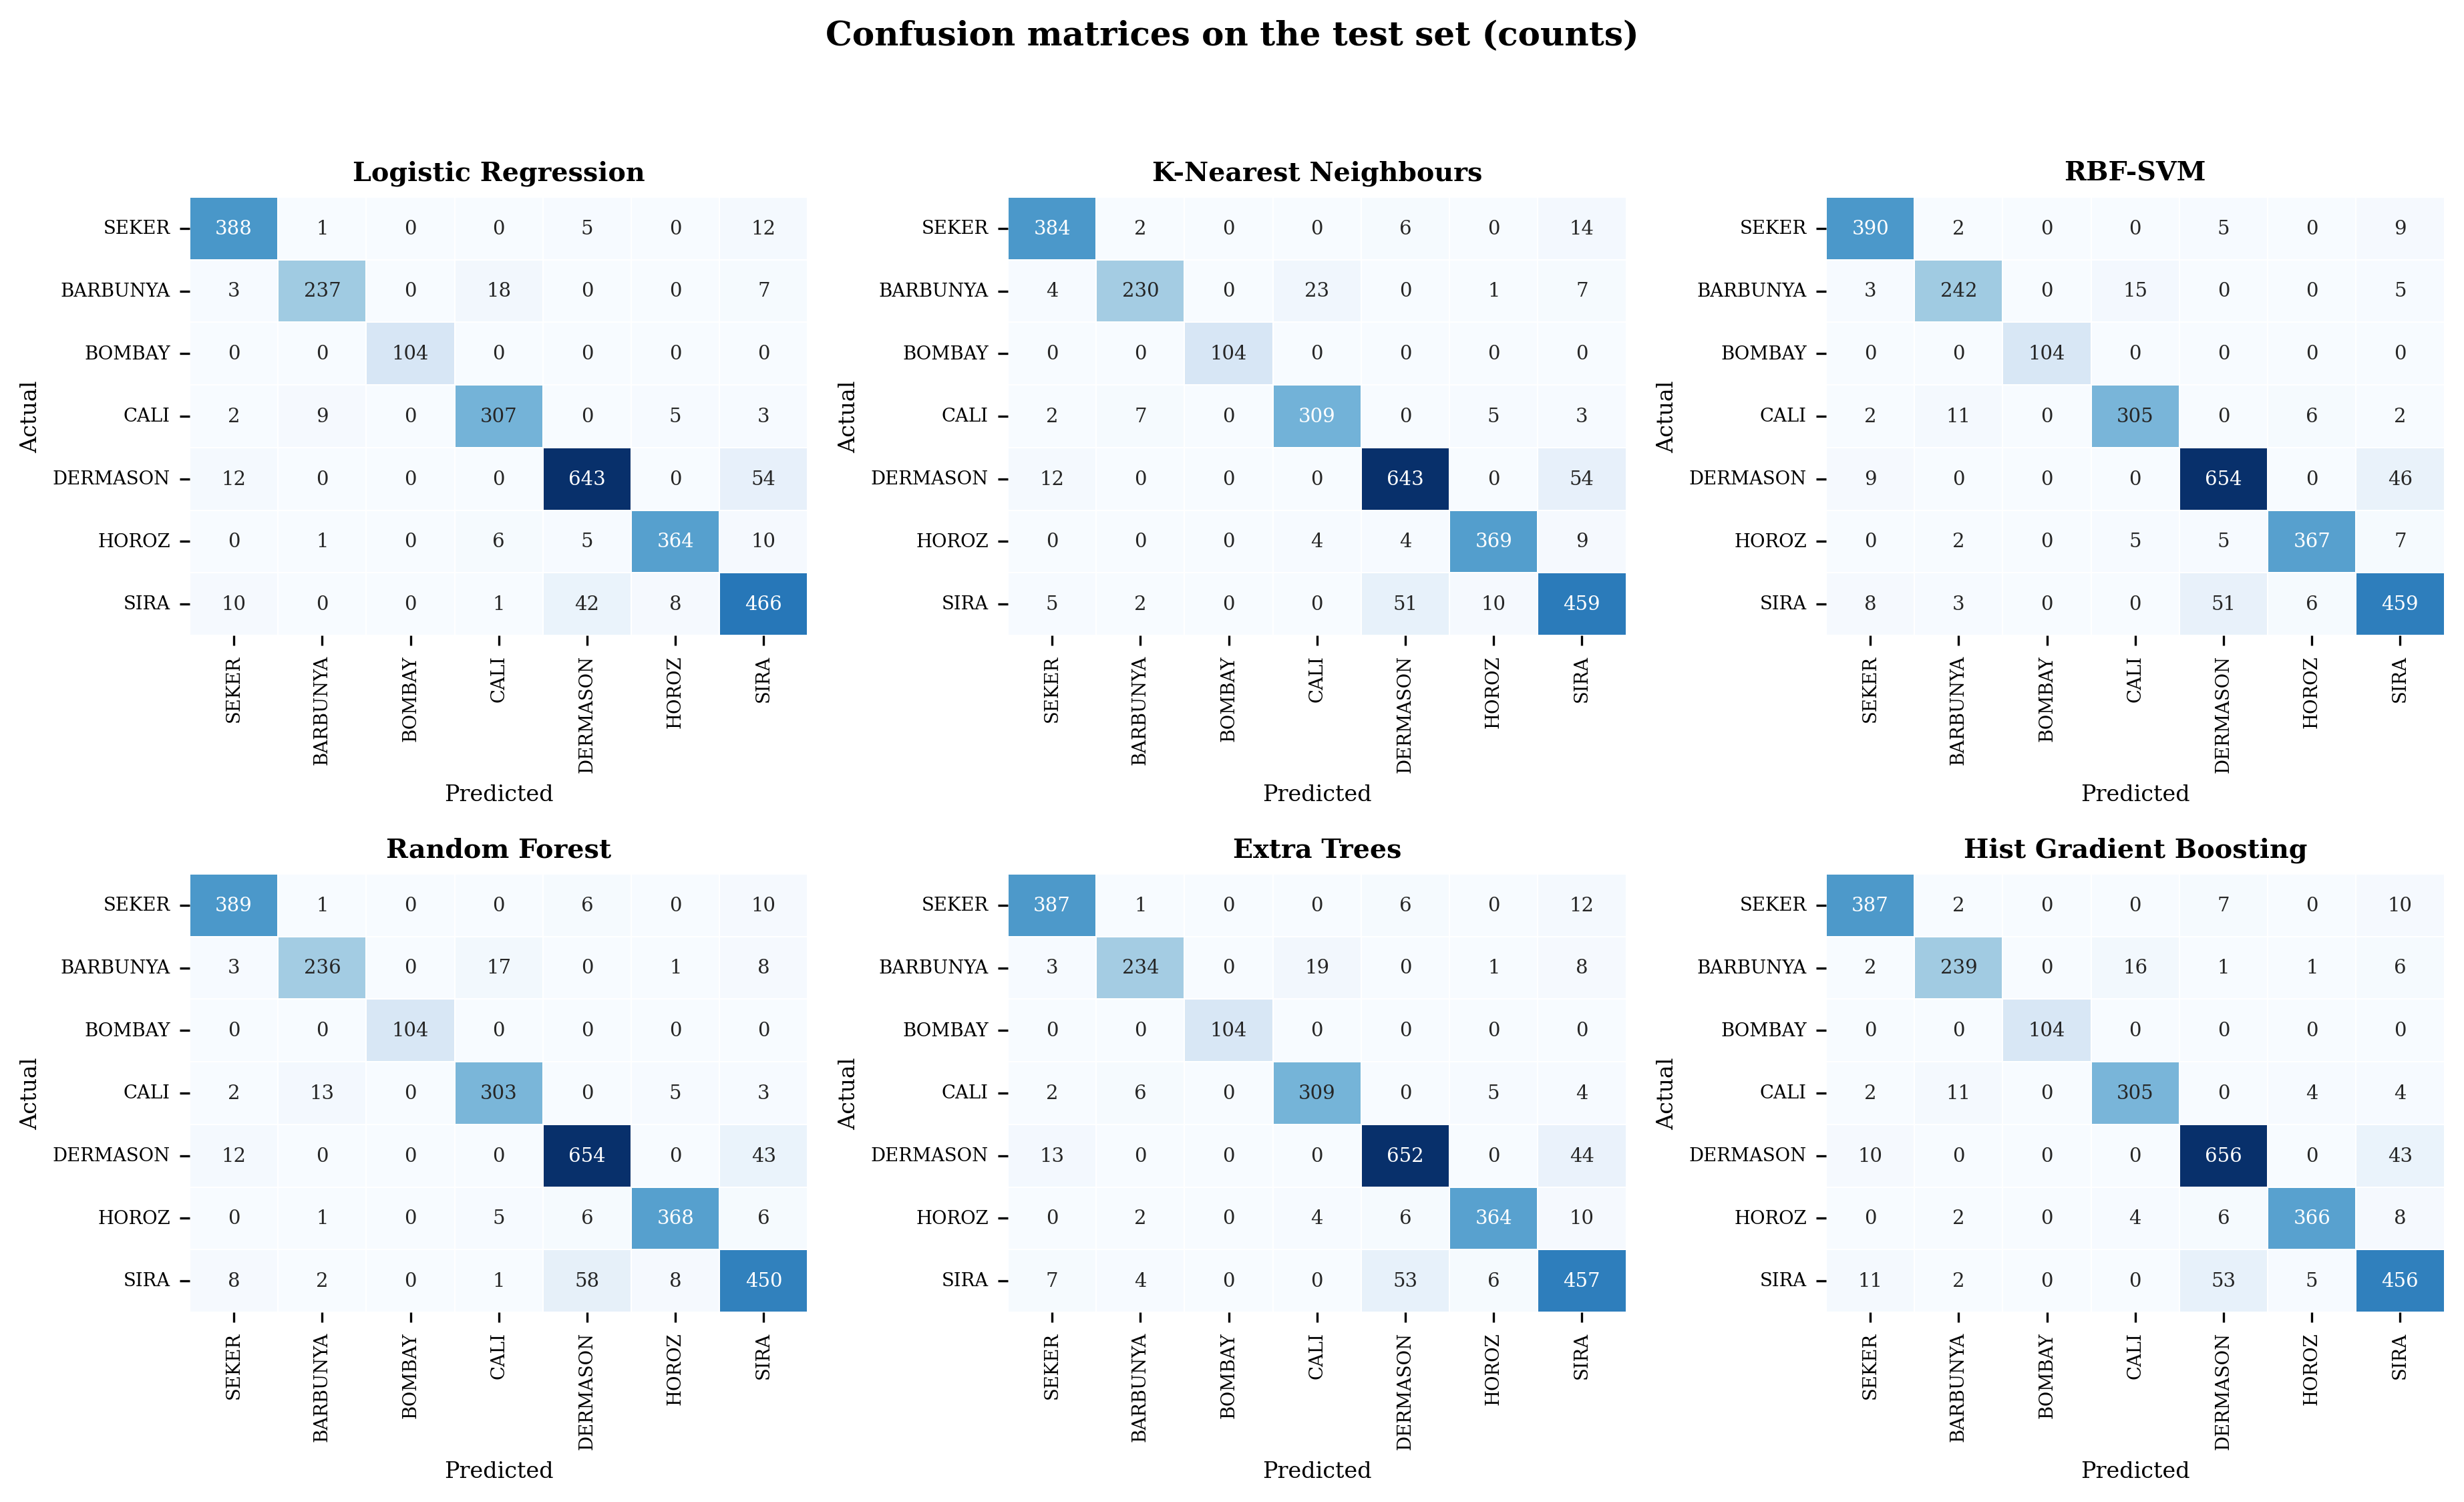
\includegraphics[width=0.94\textwidth]{fig_6_2_confusion_matrices.png}
\caption{Confusion matrices on the held-out test set. The Sira--Dermason block is
the dominant error source for every model.}
\label{fig:cmgrid}
\end{figure}

The row-normalised matrix of the selected model in Figure~\ref{fig:cmbest} makes
the magnitude explicit. Bombay, Horoz, Seker and Cali all exceed 0.93 on the
diagonal. Dermason and Sira are at 0.922 and 0.871, and the leakage between them
is 6.4\% of Dermason beans predicted as Sira and 9.7\% of Sira beans predicted as
Dermason.

\begin{figure}[htbp]
\centering
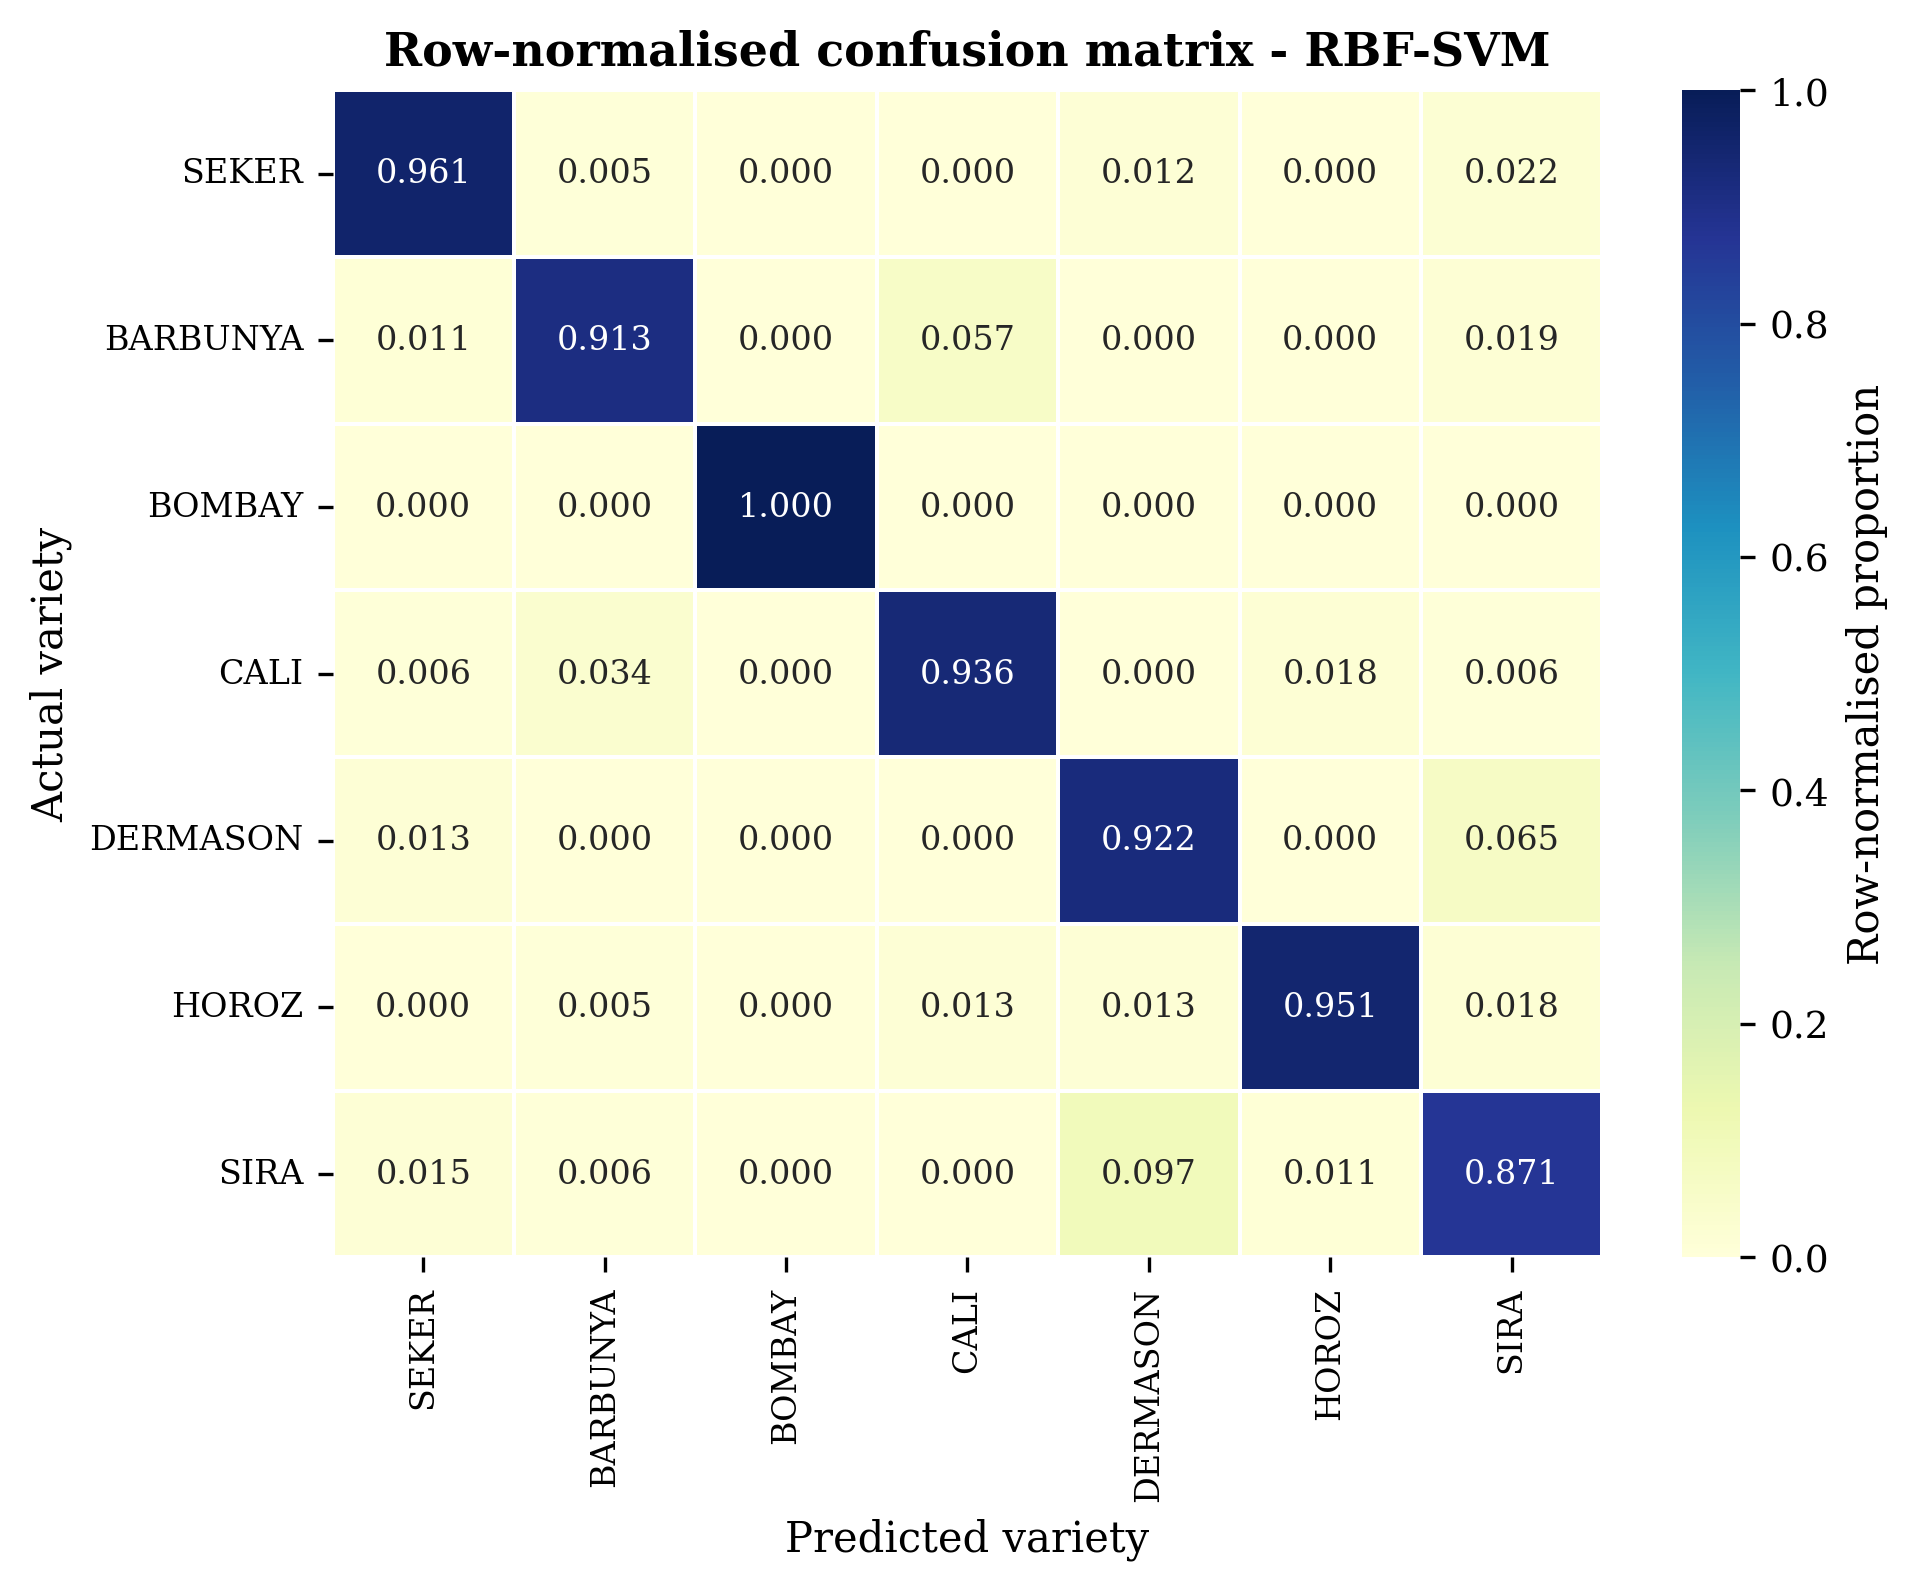
\includegraphics[width=0.58\textwidth]{fig_6_3_confusion_matrix_best.png}
\caption{Row-normalised confusion matrix of the \BestModel{}. Each row sums to
1.00; the diagonal is the per-class recall.}
\label{fig:cmbest}
\end{figure}

Table~\ref{tab:per_class} and Figure~\ref{fig:perclass} give the per-class scores.
Bombay reaches precision and recall of 1.000 on 104 test beans, which confirms the
expectation from Chapter~3 that its area separates it completely. Sira has the
lowest F1 at 0.8701, driven by a recall of 0.8710 rather than by poor precision
(0.8693), which means Sira beans are being absorbed by a neighbour rather than
being wrongly attracted into Sira. Horoz, which the EDA suggested might be
confusable, turns out to be the second-best class at 0.9595, because its extreme
compactness (0.701, the lowest of the seven) is a distinctive signal.

\begin{table}[htbp]
\centering
\small
\caption{Per-class performance of the selected model (RBF-SVM)}
\label{tab:per_class}
\begin{tabular}{lrrrr}
\toprule
Variety & Precision & Recall & F1-score & Support \\
\midrule
Seker & 0.9466 & 0.9606 & 0.9535 & 406 \\
Barbunya & 0.9308 & 0.9132 & 0.9219 & 265 \\
Bombay & 1.0000 & 1.0000 & 1.0000 & 104 \\
Cali & 0.9385 & 0.9356 & 0.9370 & 326 \\
Dermason & 0.9147 & 0.9224 & 0.9185 & 709 \\
Horoz & 0.9683 & 0.9508 & 0.9595 & 386 \\
Sira & 0.8693 & 0.8710 & 0.8701 & 527 \\
\midrule
Macro average & 0.9383 & 0.9362 & 0.9372 & 2723 \\
\bottomrule
\end{tabular}
\end{table}


\begin{figure}[htbp]
\centering
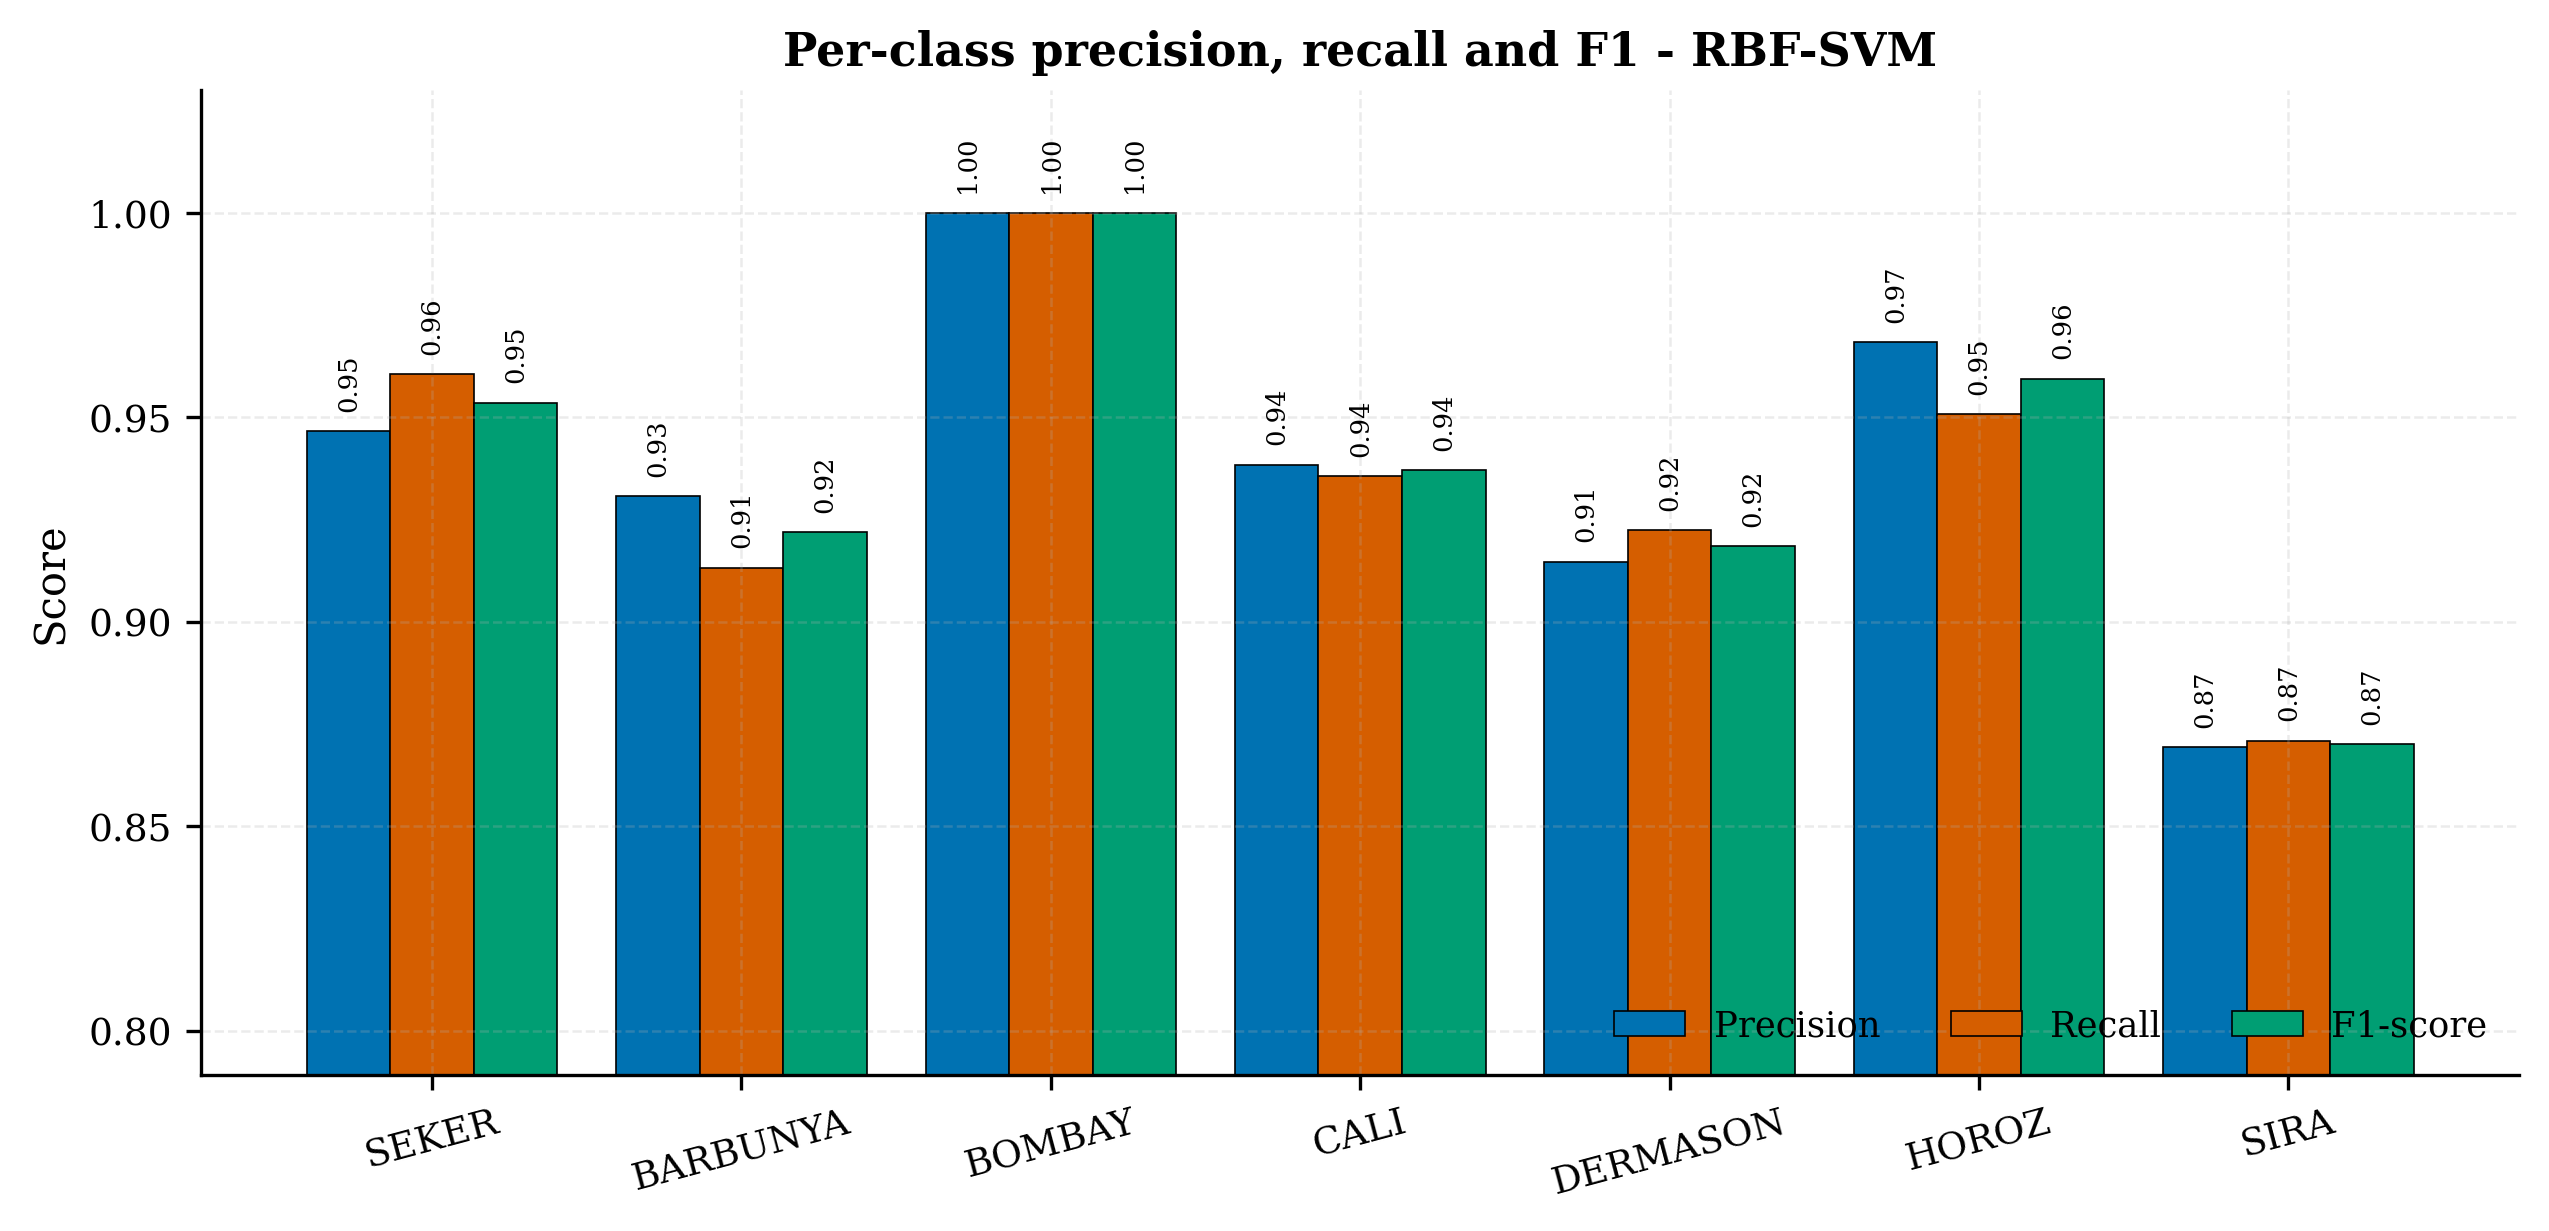
\includegraphics[width=0.78\textwidth]{fig_6_4_per_class_metrics.png}
\caption{Per-class precision, recall and F1 of the \BestModel{}. Bombay is
perfect; Sira is the weakest class.}
\label{fig:perclass}
\end{figure}

Figure~\ref{fig:roc} shows the one-vs-rest ROC curves. All seven areas exceed
0.986, and the macro average is \BestAUC. The curves confirm that the difficulty
is not in ranking beans by confidence but in the final decision at the boundary:
the model ranks a Sira bean above a Dermason bean 98.6\% of the time, yet still
misassigns 9.7\% of them once a single threshold is applied to all classes.

\begin{figure}[htbp]
\centering
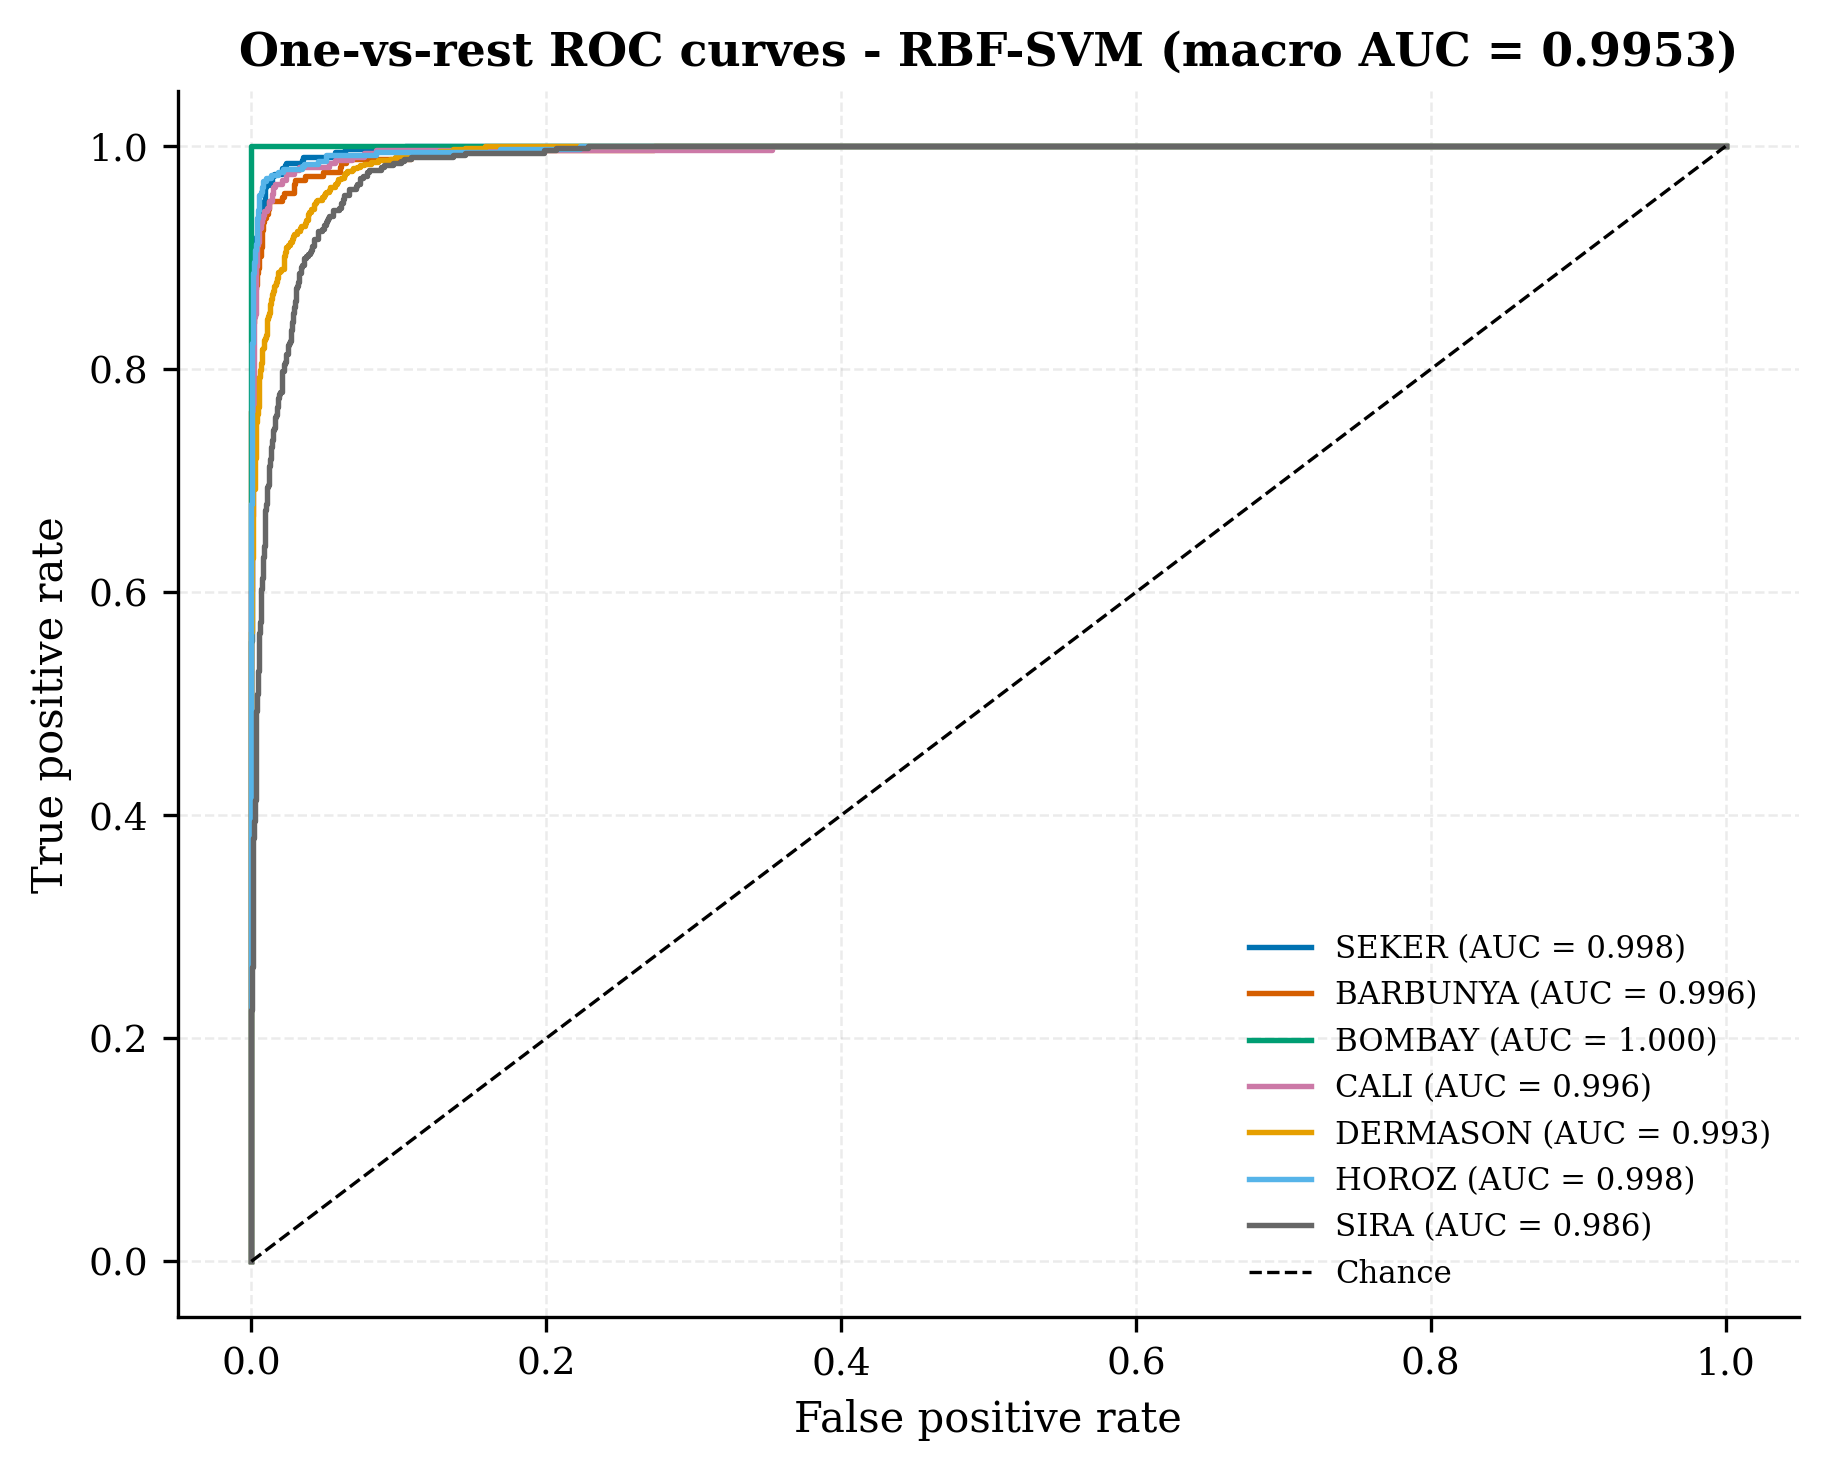
\includegraphics[width=0.58\textwidth]{fig_6_5_roc_curves.png}
\caption{One-vs-rest ROC curves for the \BestModel{}. Macro AUC is \BestAUC.}
\label{fig:roc}
\end{figure}

Figure~\ref{fig:cvdist} shows the fold-to-fold spread of the selected
configuration for each model. The boxes are narrow, between 0.003 and 0.006
wide, which indicates that the tuning is stable: none of the six models depends on
a lucky fold. It also confirms that the gap between the top five models is smaller
than their own variance.

\begin{figure}[htbp]
\centering
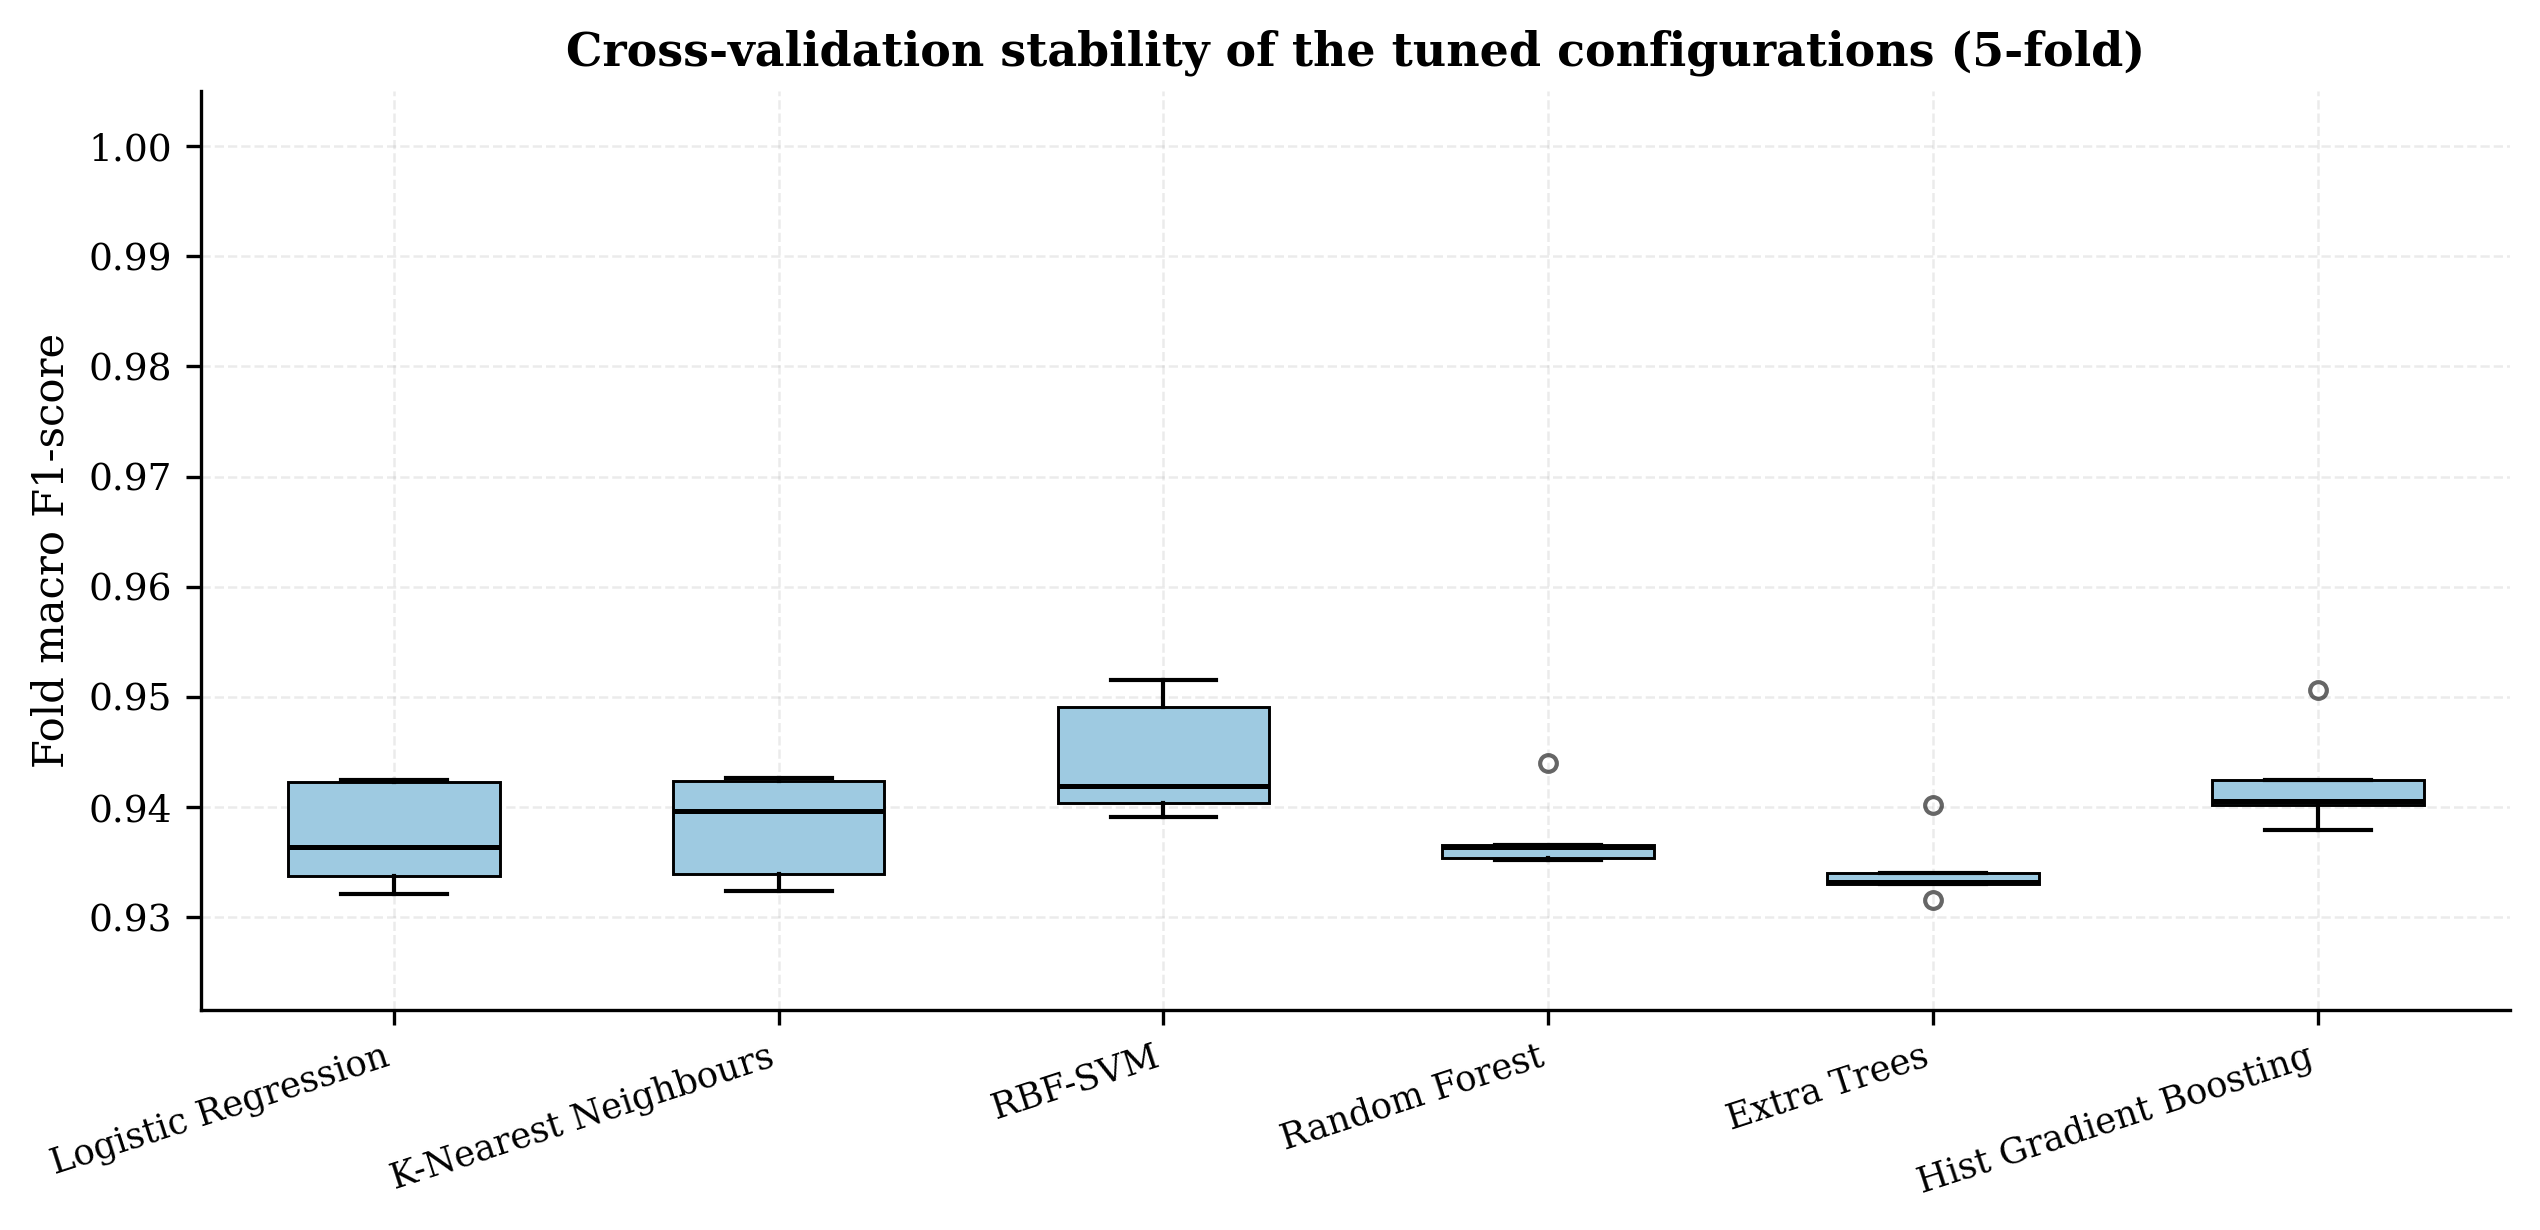
\includegraphics[width=0.78\textwidth]{fig_6_6_cv_fold_distribution.png}
\caption{Macro F1 of the selected configuration in each of the five folds. The
boxes are narrower than the gaps between adjacent models in several cases, which
limits how far the ranking can be trusted.}
\label{fig:cvdist}
\end{figure}

\section{Model Comparison and Discussion}

\textbf{Why the RBF-SVM wins.} The SVM's advantage is small but consistent: it is
first on cross-validation, first on the test set, and first on every per-class
aggregate except weighted F1, where it ties with its own accuracy. Its success is
explained by the geometry established in Chapter~3. The classes are compact and
roughly ellipsoidal, with one large separated cluster (Bombay) and one dense
overlapping cloud. An RBF kernel represents exactly that structure: a Gaussian
centred on each support vector, with $\gamma = 0.01$ setting a width comparable to
the spacing between clusters. The selected $C = 100$ is large, which means the
model is willing to accept few margin violations; with 10,888 training beans and a
well-conditioned feature space, that capacity is available without overfitting,
as the narrow cross-validation spread confirms.

\textbf{The linear baseline is closer than expected.} Logistic regression reaches
\BestFOne{} minus 0.0035 macro F1, a difference of about ten beans. This is worth
stating plainly rather than fitting to the narrative that a nonlinear kernel is
essential. After standardisation, the 16-dimensional space is close to linearly
separable for five of the seven varieties, and the remaining structure is captured
adequately by a hyperplane. The nonlinear models earn their extra complexity on a
small number of boundary beans, not by transforming the problem. A practitioner
who needed the simplest defensible model could choose logistic regression here and
lose very little.

\textbf{Why the ensembles do not win.} Random Forest, Extra Trees and histogram
gradient boosting are all within 0.006 macro F1 of the SVM, but none of them beats
it. The reason is visible in the confusion structure. Tree ensembles partition the
feature space with axis-aligned splits, so a boundary defined by a ratio such as
$A/L^3$ has to be approximated by a staircase. The varieties that are separated by
a ratio, Cali and Barbunya in particular, are therefore harder for a forest than
for a kernel that can orient its boundary arbitrarily. Extra Trees, with its
random thresholds, is slightly worse than Random Forest here, which suggests that
the extra randomisation costs more bias than it saves in variance on this feature
set.

\textbf{Why kNN is last.} kNN reaches 0.9300 macro F1 with $k = 9$ and distance
weighting, which is a respectable result for a method with no training phase. Its
weakness is the one predicted in Chapter~5: in 16 dimensions the contrast between
near and far neighbours is weak, and the dense overlapping cloud contains beans
whose nine nearest neighbours belong to three different varieties. Its ROC-AUC of
0.9870 is the lowest of the six, which confirms that the ranking itself is less
reliable, not only the threshold.

\textbf{Cost.} Figure~\ref{fig:cost} plots test macro F1 against hyperparameter
search time on a logarithmic axis. The spread in accuracy is 0.0072 while the
spread in cost is a factor of 67, from 2.7~s for logistic regression to 184~s for
Random Forest. The Random Forest search was the most expensive and produced the
fourth-best model, while the SVM search took \BestSearchS{}~s and produced the
best. At prediction time the ordering reverses: the SVM needs
\BestPredictMs{}~ms for 2,723 beans, whereas histogram gradient boosting needs
11~ms and logistic regression 0.6~ms. If throughput mattered more than the last
half-percent of macro F1, the boosted tree would be the better engineering choice.

\begin{figure}[htbp]
\centering
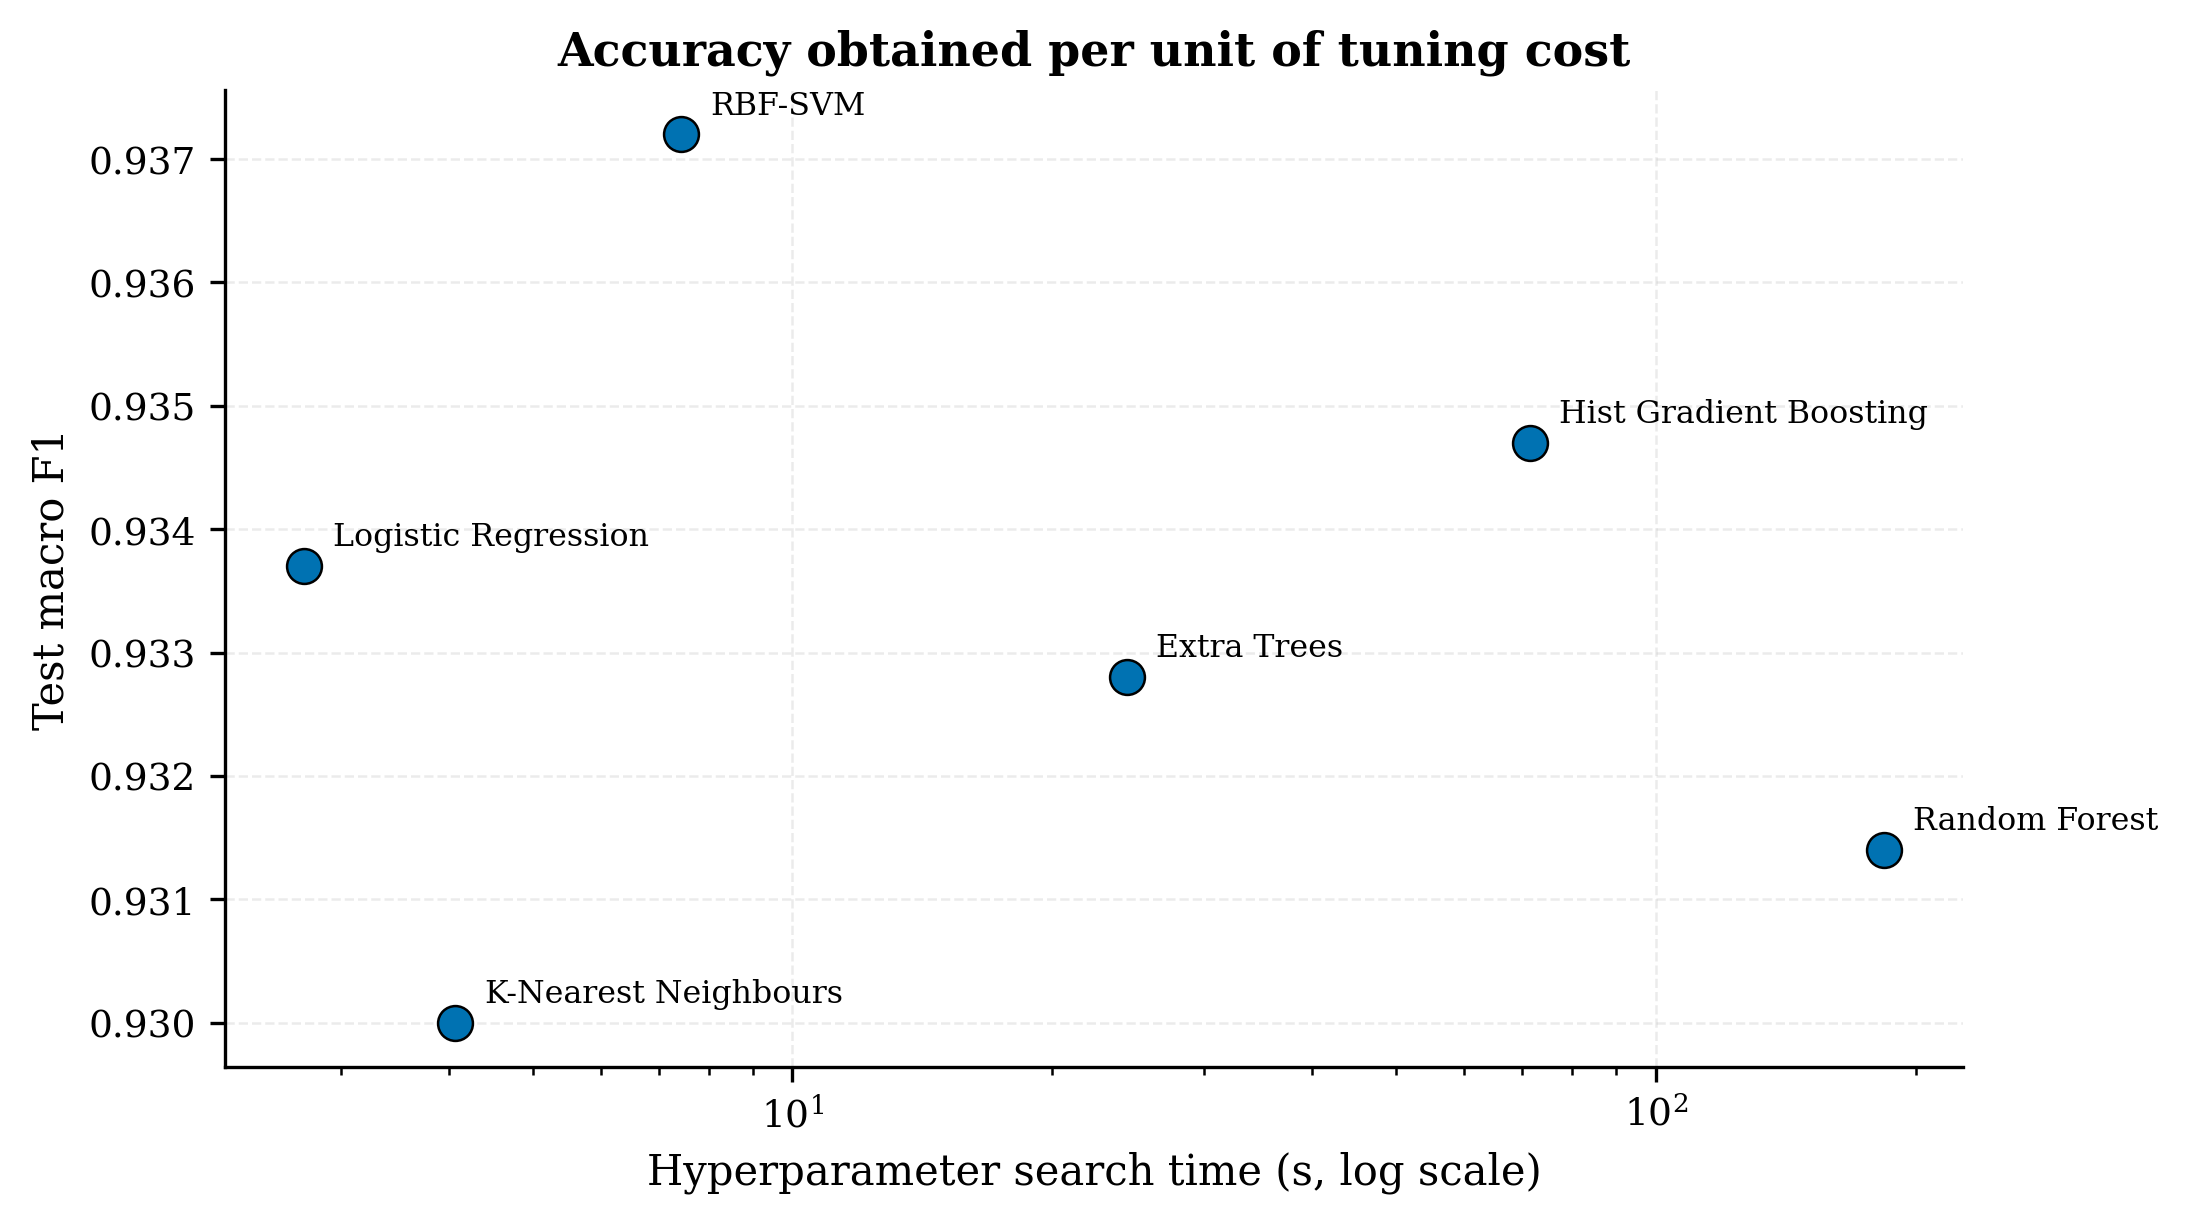
\includegraphics[width=0.66\textwidth]{fig_6_9_cost_tradeoff.png}
\caption{Test macro F1 against hyperparameter search time. Accuracy varies by
0.007 across models while cost varies by a factor of 67.}
\label{fig:cost}
\end{figure}

\textbf{Feature selection and class weighting.} Two controlled experiments
support the preprocessing decisions of Chapter~4. Dropping the five redundant size
features changes cross-validated macro F1 from \AblationFull{} to
\AblationReduced{}, an improvement smaller than the fold standard deviation, so
the 16-feature set was kept (Table~\ref{tab:ablation}). Balancing the class
weights lowers the same score from \CWNone{} to \CWBalanced{}
(Table~\ref{tab:class_weight}), so the original distribution was kept. Both results
are negative, and both are more useful than an untested assumption: they show that
the usual remedies for redundancy and imbalance do not help on this particular
dataset.

\section{Sample Predictions and Demonstration}

Table~\ref{tab:sample_predictions} shows one test bean from each variety,
classified by the saved pipeline. All seven are correct. The Bombay bean is
predicted with near-certainty, as expected from a variety separated by area alone.
The Sira bean has the lowest confidence of the seven, which is consistent with Sira
being the weakest class in Table~\ref{tab:per_class}: the model is least sure
exactly where it makes its mistakes. The full 16-feature vectors, the runner-up
class and its probability are in
\texttt{results/predictions/sample\_predictions.csv}.

\begin{table}[htbp]
\centering
\scriptsize
\caption{Representative test beans, one per variety, classified by the saved pipeline}
\label{tab:sample_predictions}
\begin{tabular}{clrrrrrrccc}
\toprule
\# & Area & Perimeter & Compactness & roundness & ShapeFactor1 & Extent & Actual & Predicted & Correct & P(max) \\
\midrule
1 & 41,586 & 745 & 0.8772 & 0.9403 & 0.0063 & 0.7438 & Seker & Seker & Yes & 0.994 \\
2 & 71,236 & 1,055 & 0.8705 & 0.8037 & 0.0049 & 0.8264 & Barbunya & Barbunya & Yes & 1.000 \\
3 & 152,884 & 1,470 & 0.8433 & 0.8896 & 0.0034 & 0.7761 & Bombay & Bombay & Yes & 0.999 \\
4 & 94,276 & 1,161 & 0.7775 & 0.8791 & 0.0047 & 0.8272 & Cali & Cali & Yes & 0.987 \\
5 & 37,349 & 718 & 0.8215 & 0.9115 & 0.0071 & 0.7346 & Dermason & Dermason & Yes & 0.723 \\
6 & 45,473 & 835 & 0.7163 & 0.8204 & 0.0074 & 0.7841 & Horoz & Horoz & Yes & 0.959 \\
7 & 43,550 & 790 & 0.7685 & 0.8764 & 0.0070 & 0.7828 & Sira & Sira & Yes & 0.936 \\
\bottomrule
\end{tabular}
\end{table}


The demonstration interface loads \texttt{models/best\_model.joblib}, which is the
scaler and the classifier as a single pipeline, so the caller supplies raw
measurements and receives a variety label with its top-three probabilities:

\begin{verbatim}
$ python -m src.predict --csv results/predictions/sample_predictions.csv
bean 1: SEKER [confidence 0.981]
        top-3: SEKER (0.981), DERMASON (0.014), SIRA (0.003)
bean 2: BARBUNYA [confidence 0.967]
        top-3: BARBUNYA (0.967), CALI (0.021), SIRA (0.007)
...
\end{verbatim}

\section{Error Analysis}

\TestErrors{} of the \TestRows{} test beans were misclassified, a rate of
\TestErrorPct\%. Figure~\ref{fig:errors} isolates the off-diagonal counts and the
per-class error rate. The errors are not spread evenly. Sira and Dermason account
for 97 of the 202 errors, in both directions: \TopConfusion{} in \TopConfusionN{}
cases and Dermason predicted as Sira in 46. The next largest pair is Barbunya
predicted as Cali (15) together with the reverse (11). Table~\ref{tab:confusion_pairs}
lists the six largest pairs; together they account for 141 of the 202 errors, so
70\% of the failure is concentrated in three variety pairs.

\begin{table}[htbp]
\centering
\small
\caption{Most frequent confusions produced by the selected model}
\label{tab:confusion_pairs}
\begin{tabular}{lrr}
\toprule
Actual variety & Predicted as & Beans \\
\midrule
Sira & Dermason & 51 \\
Dermason & Sira & 46 \\
Barbunya & Cali & 15 \\
Cali & Barbunya & 11 \\
Seker & Sira & 9 \\
Dermason & Seker & 9 \\
\bottomrule
\end{tabular}
\end{table}


\begin{figure}[htbp]
\centering
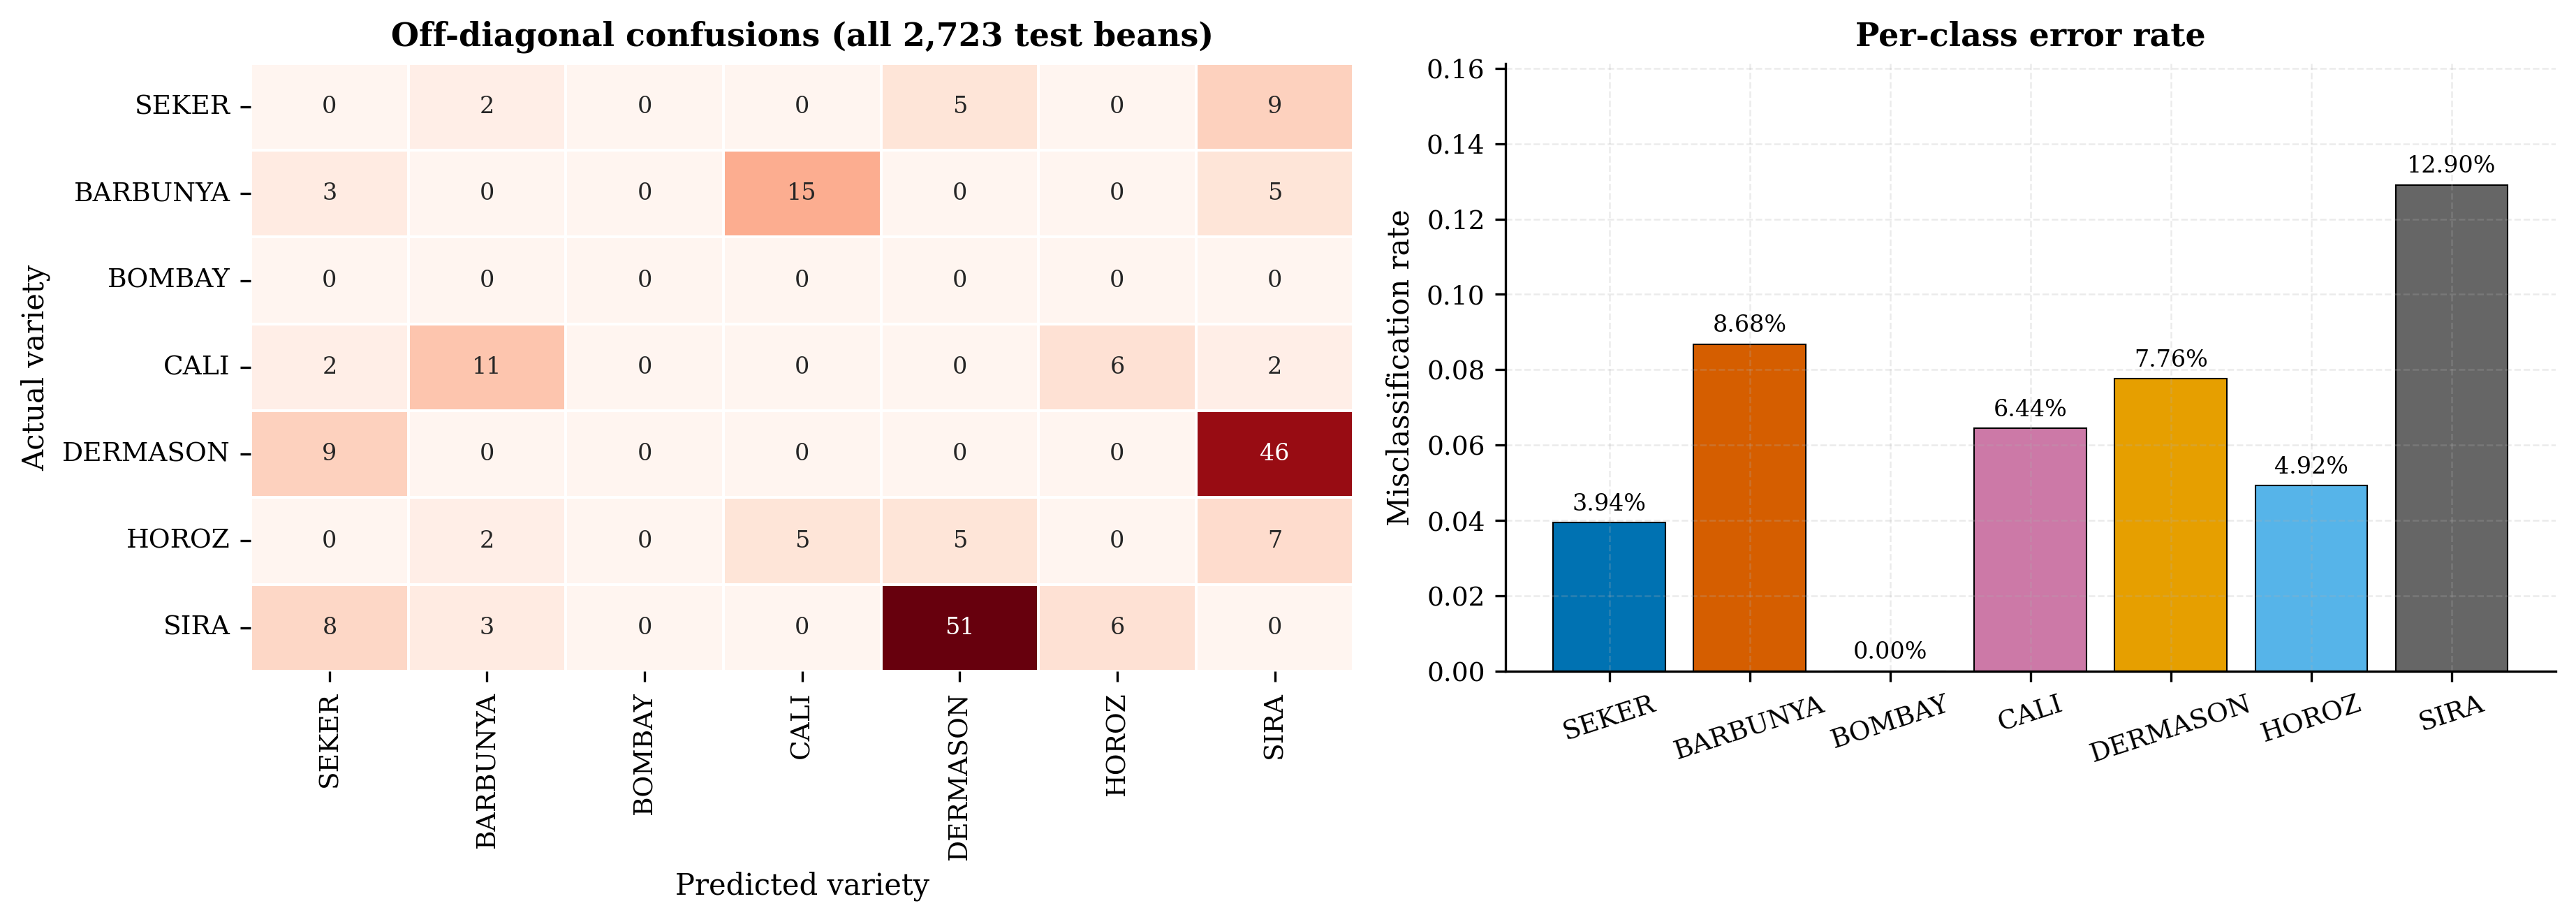
\includegraphics[width=0.92\textwidth]{fig_6_7_error_analysis.png}
\caption{Left: off-diagonal confusions of the \BestModel{}. Right: per-class
misclassification rate. Sira and Dermason dominate both panels.}
\label{fig:errors}
\end{figure}

Figure~\ref{fig:misclassified} places the misclassified beans in two feature
planes against the correctly classified ones. The pattern is unambiguous. In the
size--shape plane the errors form a band along the ridge where Dermason and Sira
meet, at areas between roughly 30,000 and 50,000 pixels and ShapeFactor1 between
0.006 and 0.008. In the compactness--roundness plane the same beans sit in the
middle of the dense cloud rather than at its edges, which is the signature of
genuine class overlap rather than of a badly placed boundary: these are beans
whose measurements are consistent with either label.

\begin{figure}[htbp]
\centering
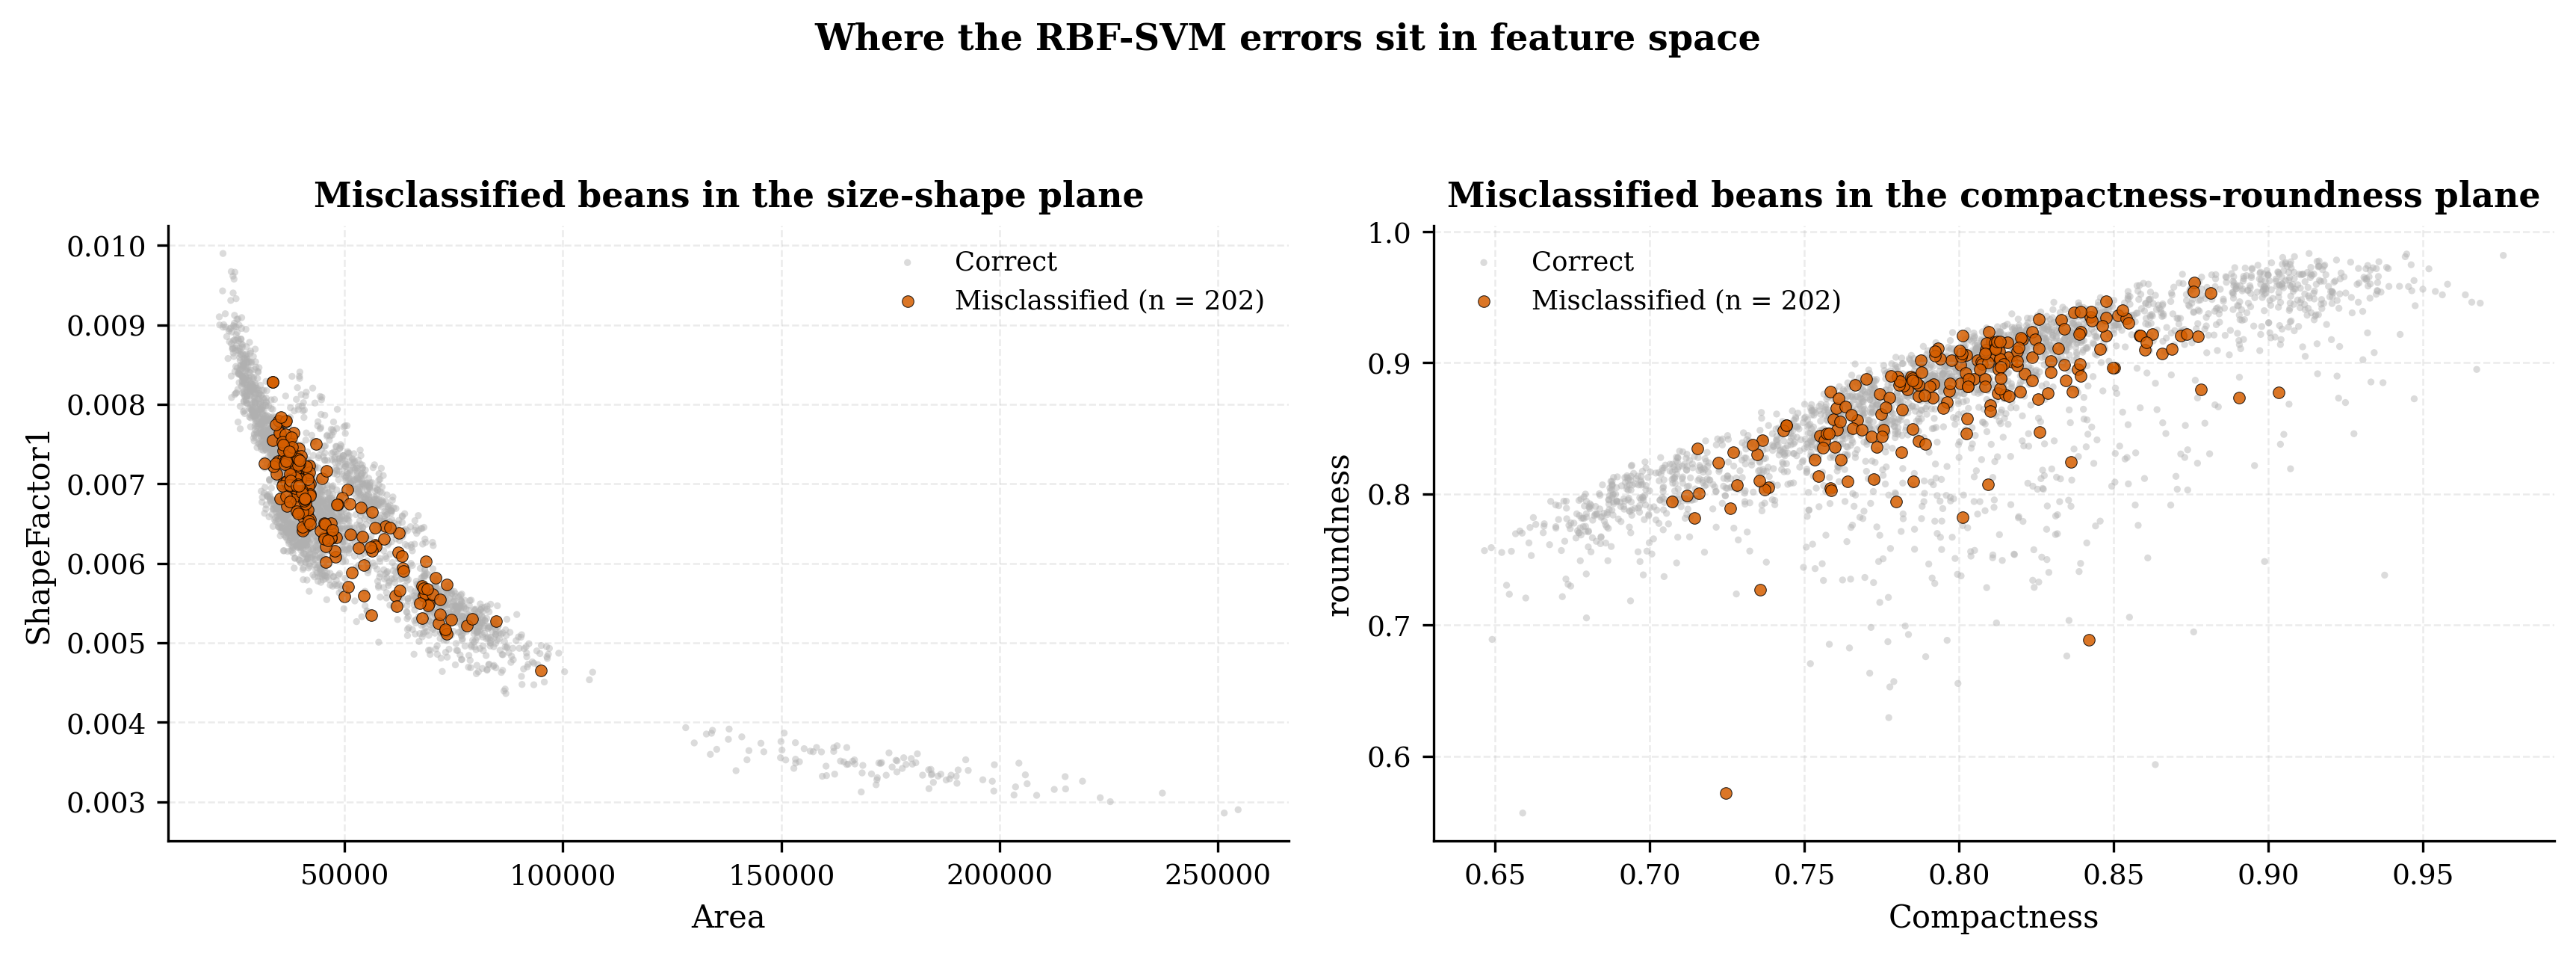
\includegraphics[width=0.92\textwidth]{fig_6_8_misclassified_scatter.png}
\caption{Misclassified test beans (orange) against correctly classified ones
(grey). The errors concentrate where the Dermason and Sira distributions meet.}
\label{fig:misclassified}
\end{figure}

The Barbunya--Cali confusion has a different cause. The two varieties have almost
the same area (69,804 and 75,538 pixels) and differ mainly in compactness, 0.805
against 0.757. That is a ratio of two measured lengths, so a small error in either
axis length moves a bean across the boundary. This is the case where an additional
descriptor, such as colour, would help most.

\section{Interpretation}

Table~\ref{tab:permutation} and Figure~\ref{fig:permutation} report permutation
importance for the selected model: each feature is shuffled in the test set and the
resulting drop in macro F1 is recorded over eight repeats. \TopPermFeature{} is
first, with a drop of \TopPermDrop{}, followed by ShapeFactor4 and AspectRation.
The ranking is plausible geometrically: roundness is $4\pi A/P^2$, the most direct
measure of how far a bean departs from a circle, and it separates Seker (0.945)
from Horoz (0.794).

\begin{table}[htbp]
\centering
\footnotesize
\caption{Permutation importance on the test set (8 repeats per feature)}
\label{tab:permutation}
\begin{tabular}{clrr}
\toprule
Rank & Feature & Drop in macro F1 & Std. dev. \\
\midrule
1 & roundness & 0.1012 & 0.0041 \\
2 & ShapeFactor4 & 0.0932 & 0.0051 \\
3 & AspectRation & 0.0530 & 0.0046 \\
4 & ShapeFactor1 & 0.0388 & 0.0013 \\
5 & MinorAxisLength & 0.0332 & 0.0034 \\
6 & Eccentricity & 0.0282 & 0.0026 \\
7 & Perimeter & 0.0282 & 0.0027 \\
8 & EquivDiameter & 0.0244 & 0.0022 \\
9 & ConvexArea & 0.0231 & 0.0025 \\
10 & Area & 0.0227 & 0.0024 \\
11 & MajorAxisLength & 0.0210 & 0.0027 \\
12 & ShapeFactor3 & 0.0199 & 0.0023 \\
13 & Compactness & 0.0181 & 0.0026 \\
14 & Solidity & 0.0169 & 0.0026 \\
15 & ShapeFactor2 & 0.0046 & 0.0020 \\
16 & Extent & 0.0038 & 0.0021 \\
\bottomrule
\end{tabular}
\end{table}


\begin{figure}[htbp]
\centering
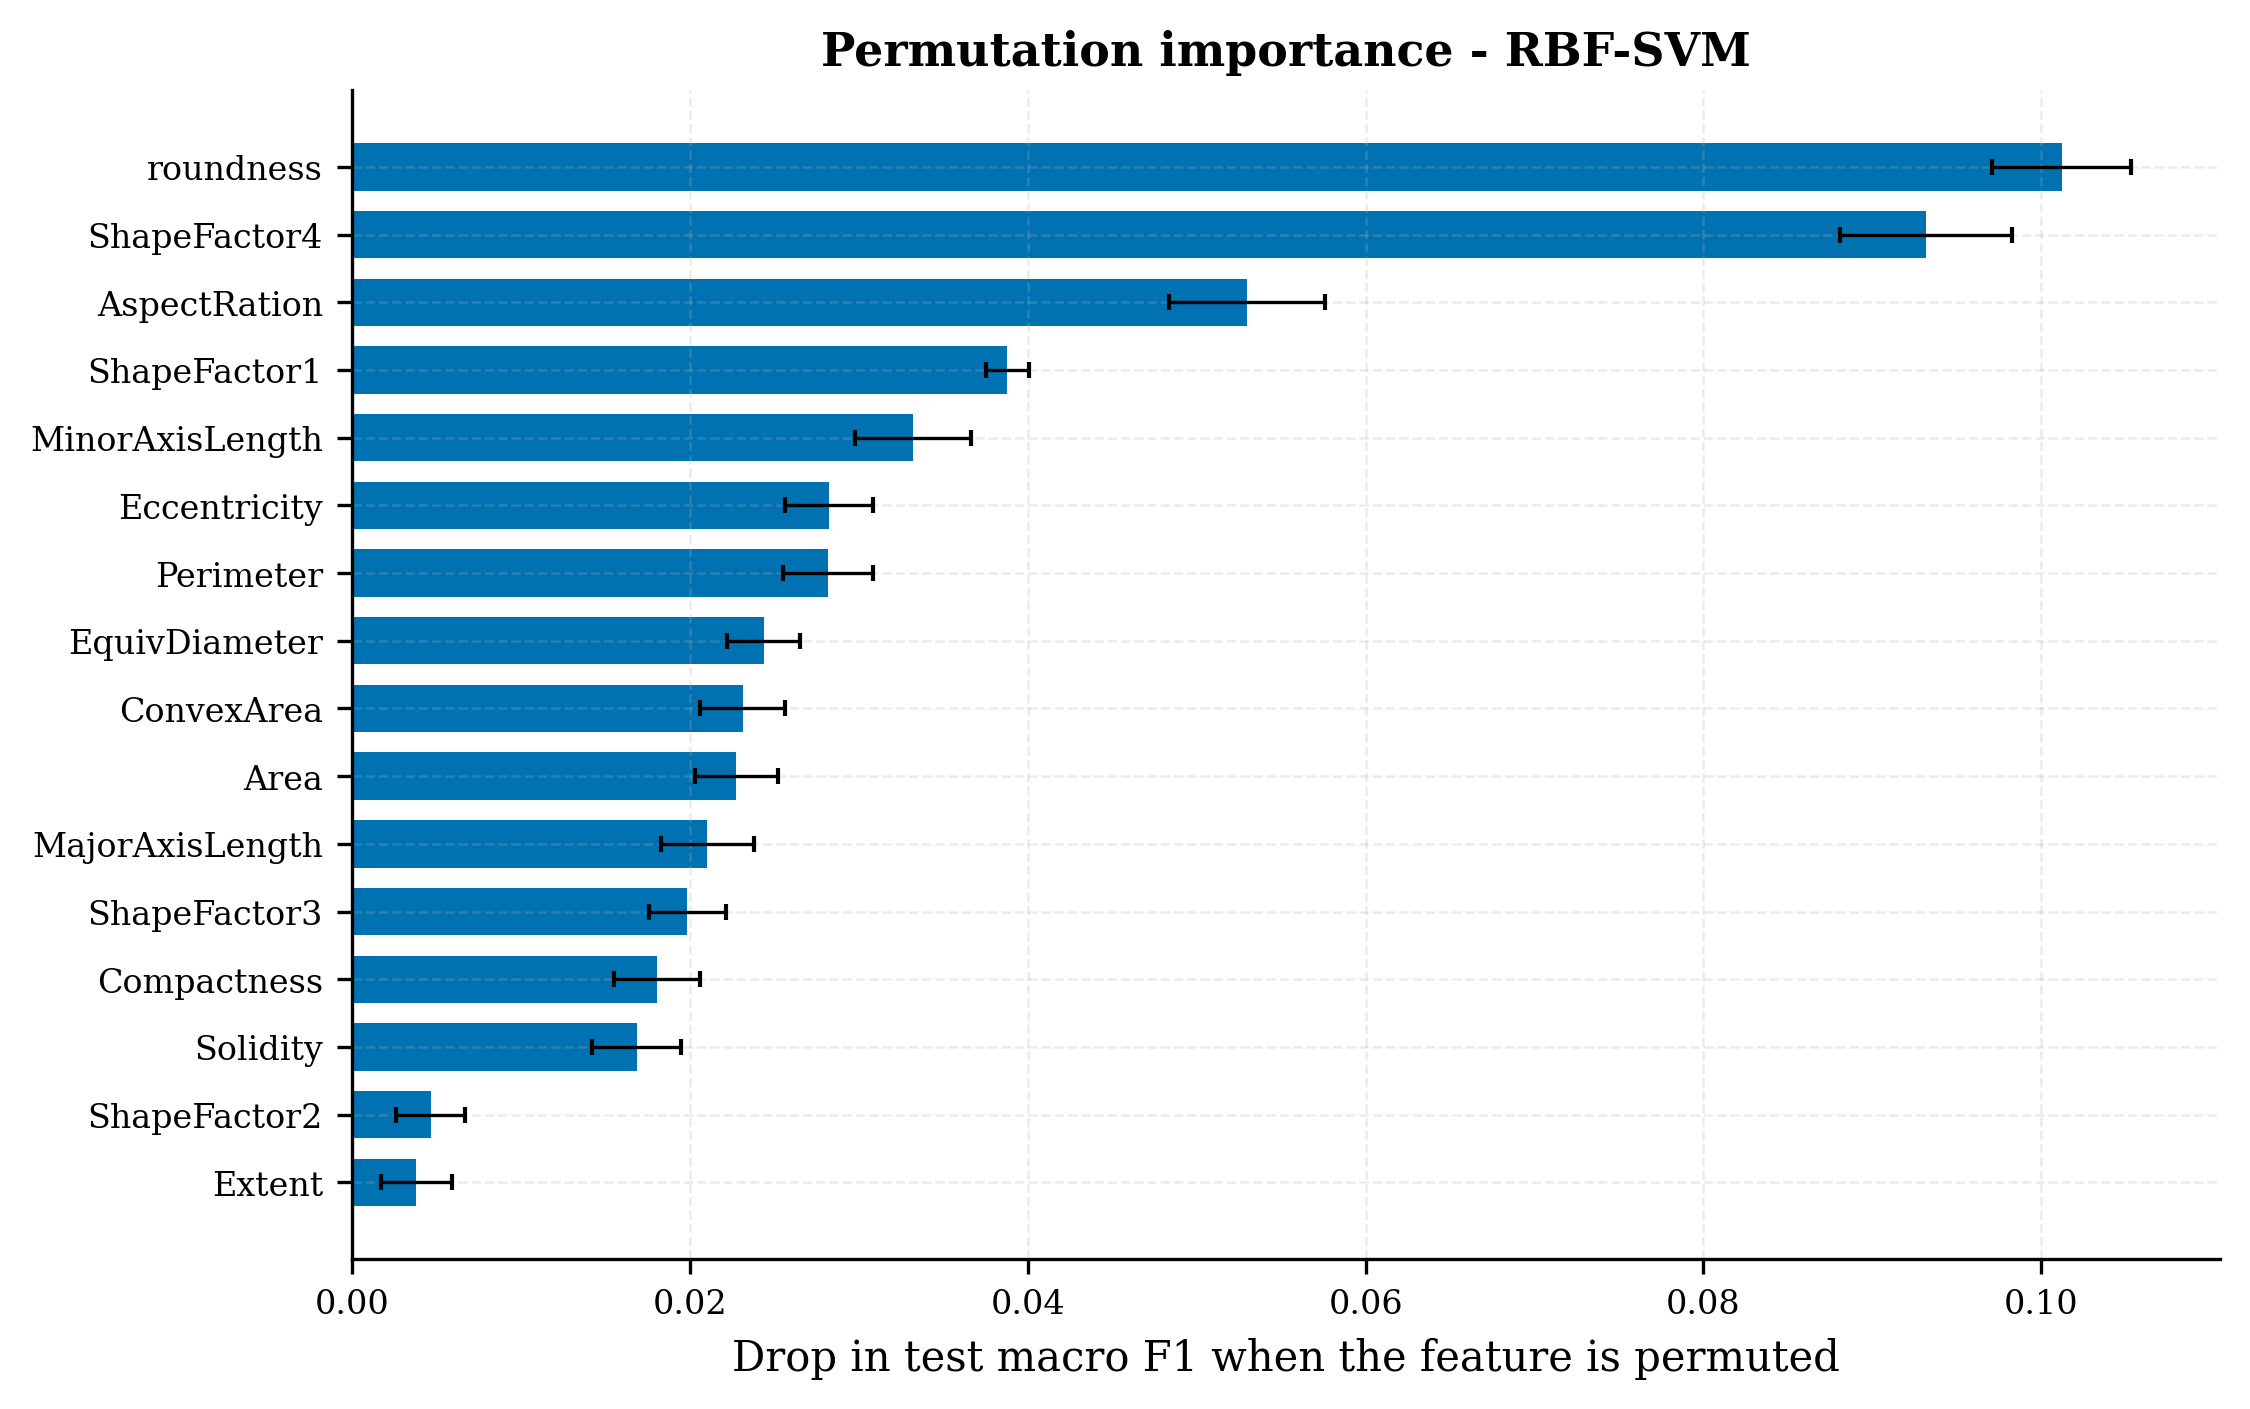
\includegraphics[width=0.64\textwidth]{fig_6_10_permutation_importance.png}
\caption{Permutation importance of the \BestModel{} on the test set. Error bars
are one standard deviation over eight repeats.}
\label{fig:permutation}
\end{figure}

Figure~\ref{fig:treeimp} shows the impurity-based importance of the two forests,
and Figure~\ref{fig:shap} shows SHAP values \cite{lundberg2017} for the Extra
Trees model, which is the
only tree ensemble for which exact TreeSHAP is cheap enough to run on 400 test
beans. The three measures do not agree. Permutation importance ranks
\TopPermFeature{} first; impurity importance and SHAP both put the size features
and ShapeFactor1 at the top.

This disagreement is expected and is itself informative. Impurity importance
measures how often a feature is used to split, and it is biased towards features
with many distinct values, which favours the continuous size measurements. SHAP
distributes credit among correlated features according to the order in which they
enter the model, so when \texttt{Perimeter} and \texttt{EquivDiameter} carry the
same information ($r = 0.99$), the first one absorbs most of the credit. Permutation
importance is the most conservative of the three, because shuffling one member of a
correlated pair leaves the other intact and the model can still recover, which is
why no single feature shows a large drop.

\begin{table}[htbp]
\centering
\small
\caption{Per-class ROC-AUC of the selected model on the test set}
\label{tab:roc_class}
\begin{tabular}{lr}
\toprule
Variety & One-vs-rest ROC-AUC \\
\midrule
Seker & 0.9982 \\
Barbunya & 0.9959 \\
Bombay & 1.0000 \\
Cali & 0.9964 \\
Dermason & 0.9928 \\
Horoz & 0.9976 \\
Sira & 0.9862 \\
\bottomrule
\end{tabular}
\end{table}


\begin{figure}[htbp]
\centering
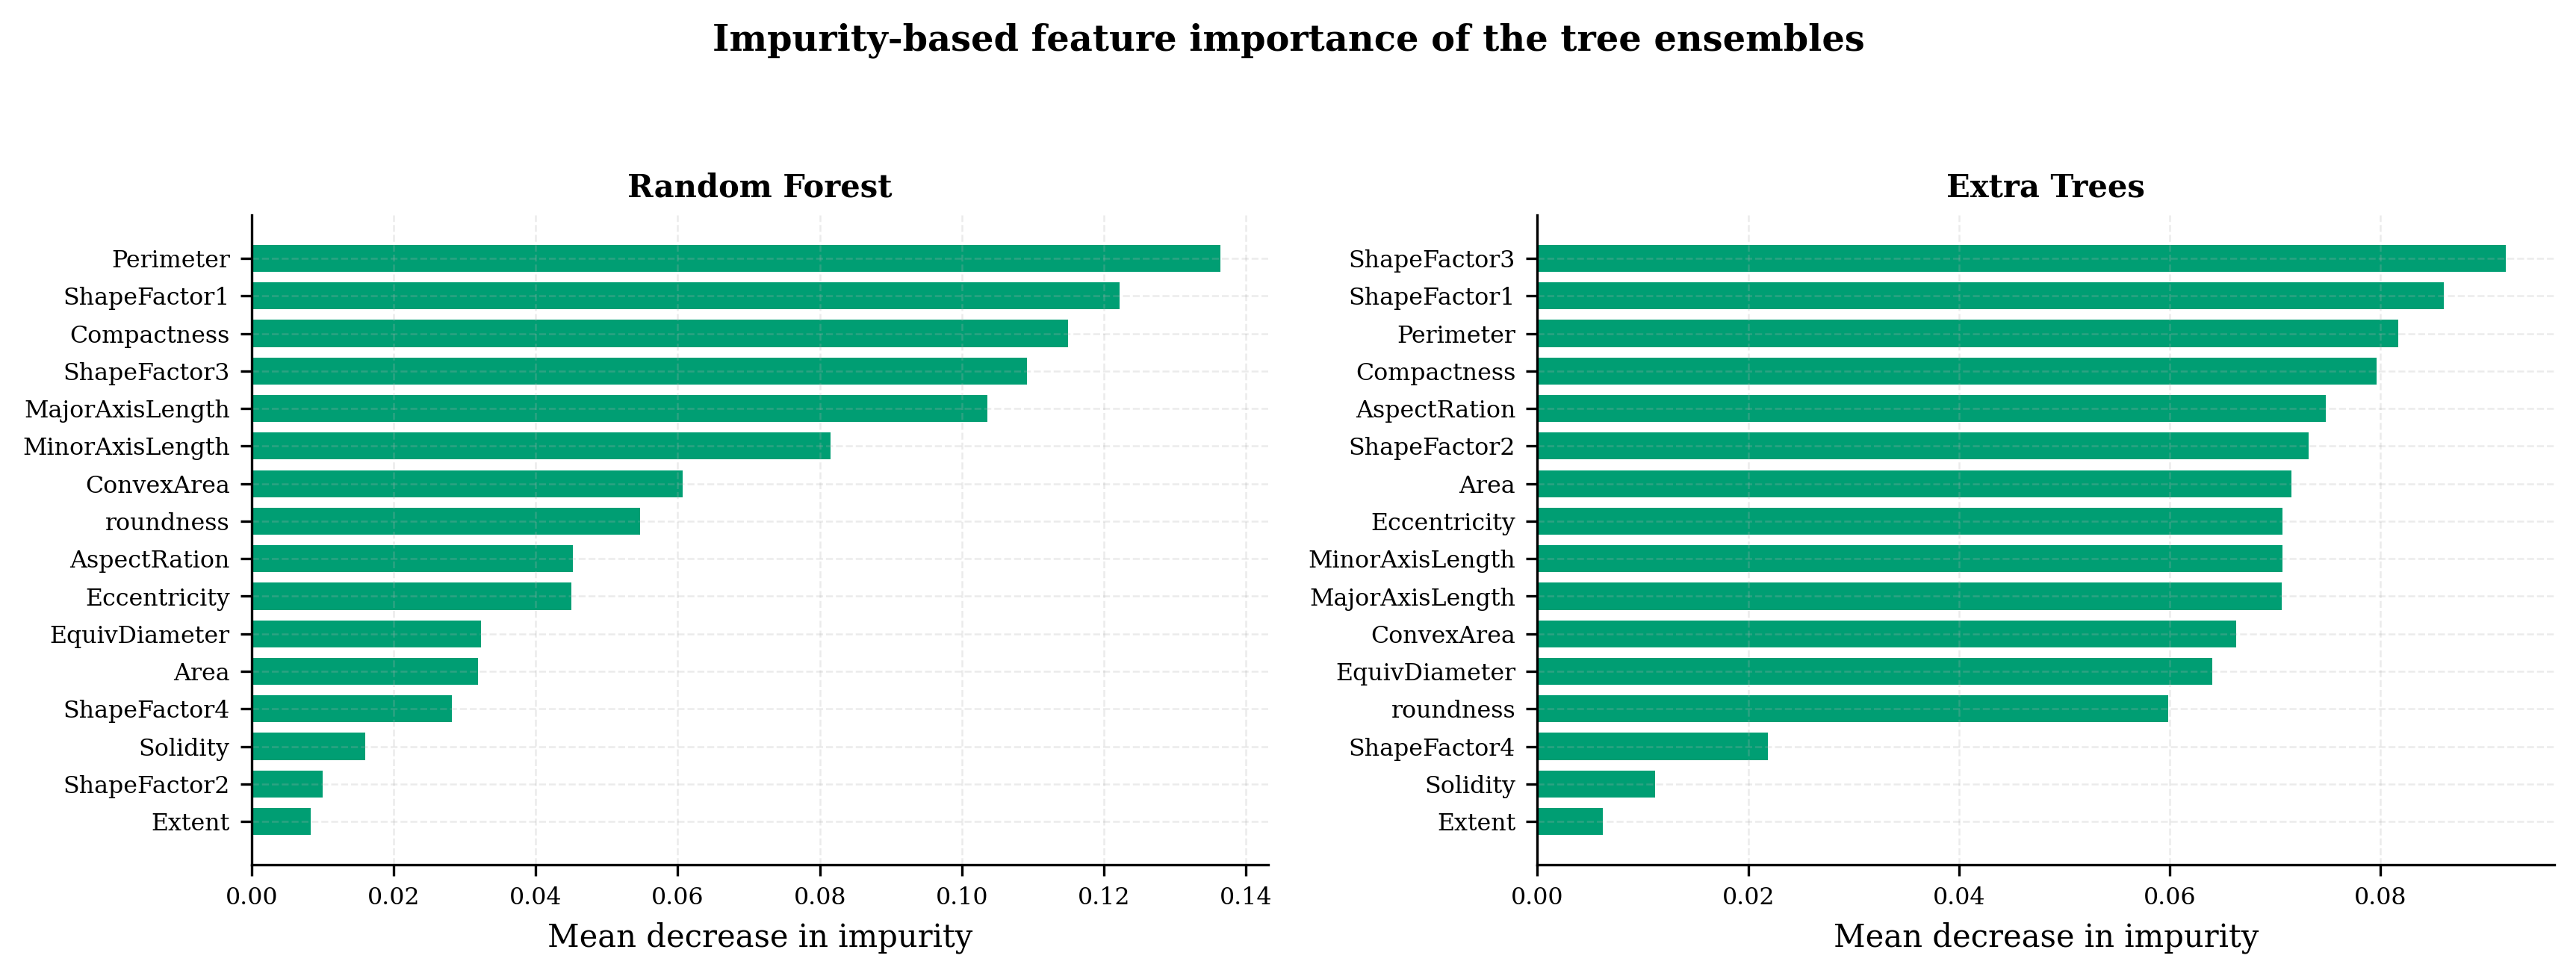
\includegraphics[width=0.92\textwidth]{fig_6_11_tree_feature_importance.png}
\caption{Impurity-based feature importance for Random Forest and Extra Trees. The
size features dominate because they are used most often for splitting.}
\label{fig:treeimp}
\end{figure}

\begin{figure}[htbp]
\centering
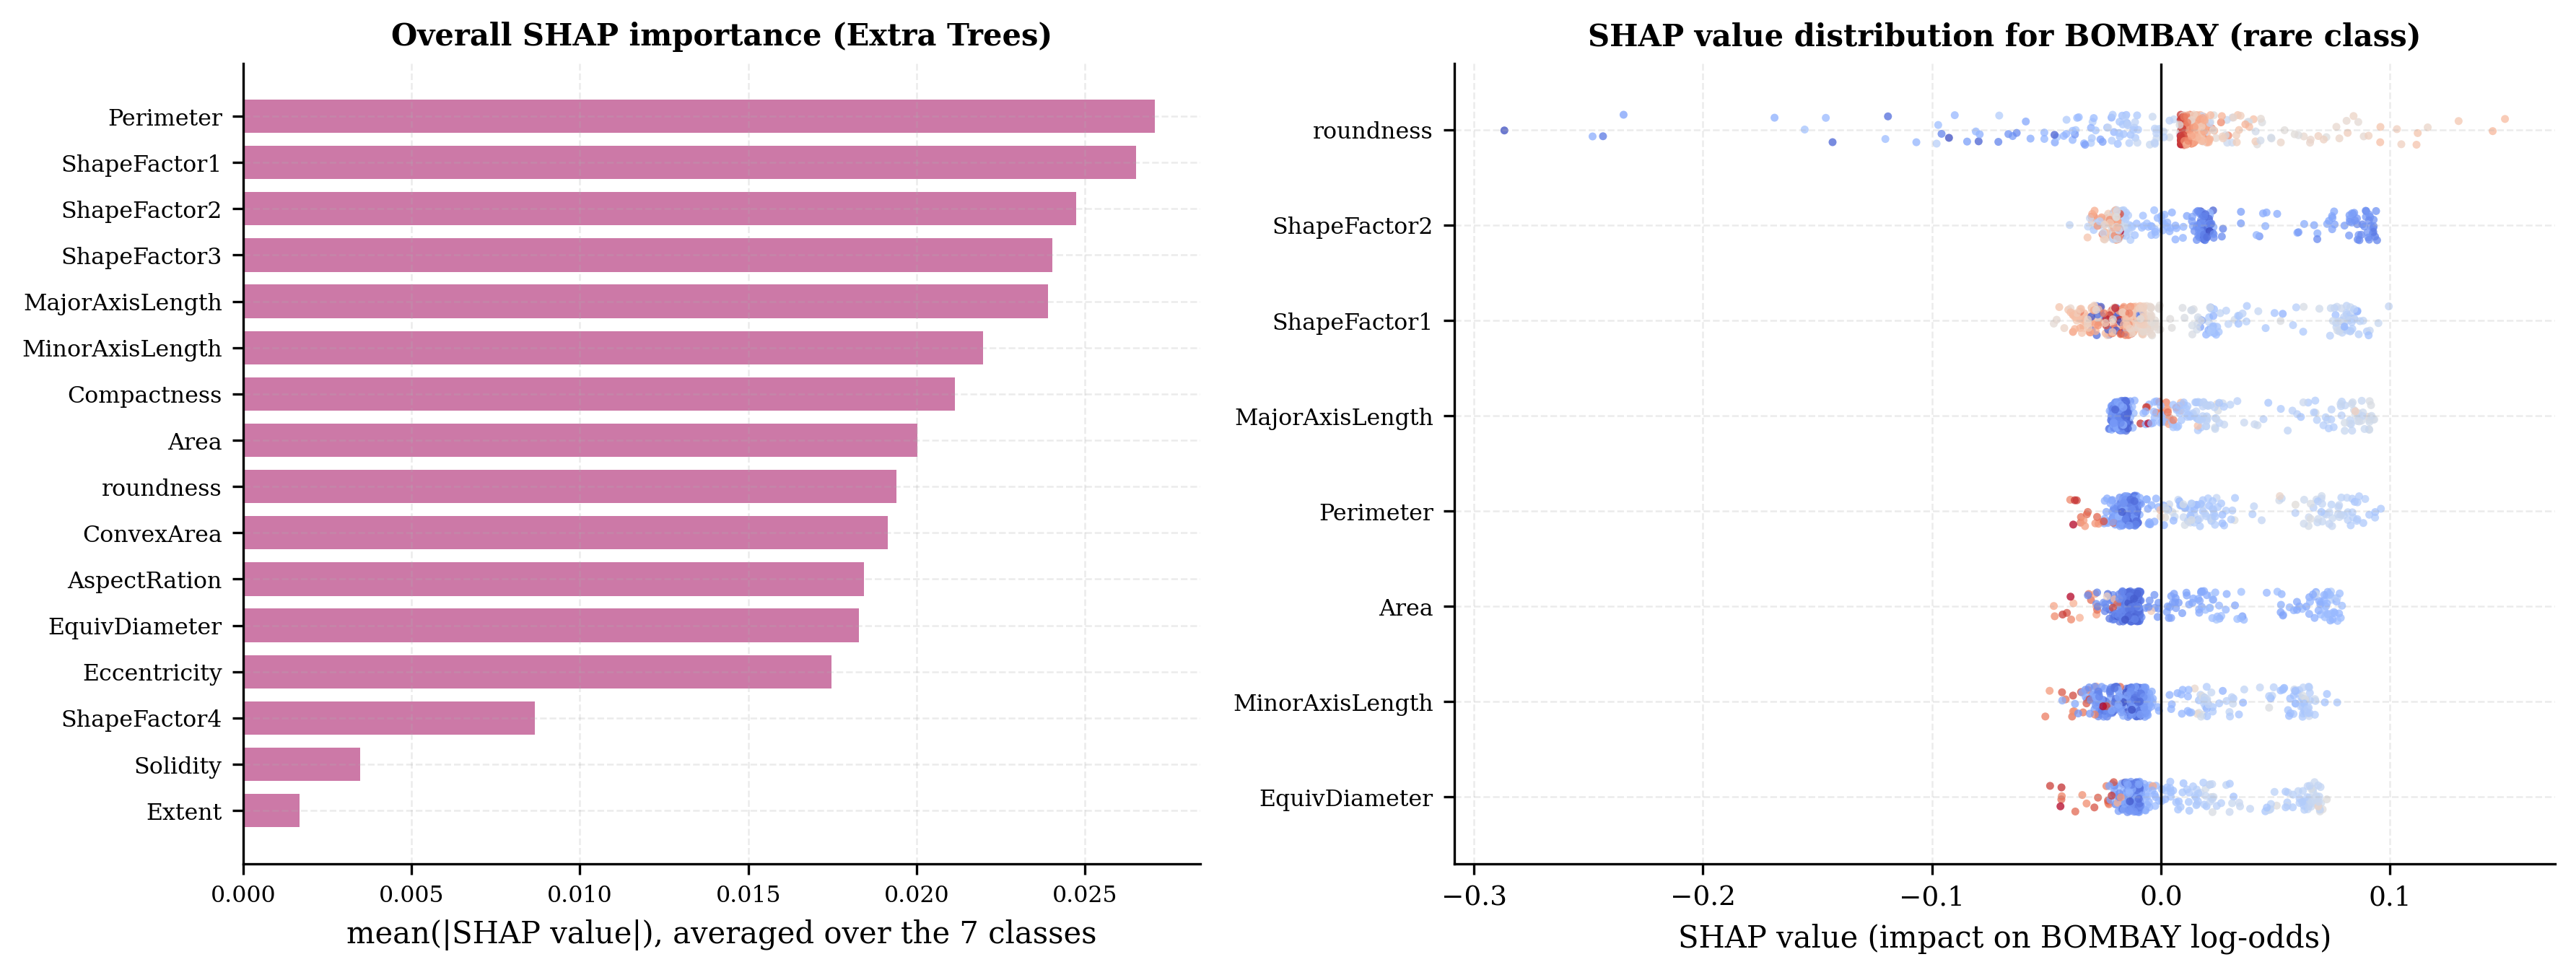
\includegraphics[width=0.94\textwidth]{fig_6_12_shap_summary.png}
\caption{SHAP analysis of the Extra Trees model. Left: mean absolute SHAP value
across the seven classes. Right: SHAP distribution for Bombay, the minority class.}
\label{fig:shap}
\end{figure}

Two cautions follow. First, none of these measures is causal. A high rank for
roundness means the fitted model relies on it, not that roundness determines the
variety; a bean's variety determines its geometry, not the reverse. Second,
because 21 feature pairs correlate above 0.90, any attribution among them is
arbitrary, and a different random seed for the forest can reorder the top five.
The stable conclusion across all three measures is only that the shape ratios and
the size features matter together, which is what the exploratory analysis
predicted and what the confusion structure confirms: size separates Bombay and
Dermason from the rest, and shape separates the varieties inside the remaining
cloud.
